%%%%%%%%%%%%%%%%%%%%%%%%%%%%%%%%%%%%%%%%%%%%%%%%%%%%%%%%%%%%%%%%%%%%%%%%%%%
%
% Generic template for TFC/TFM/TFG/Tesis
%
% $Id: book.tex,v 1.13 2014/01/11 23:27:55 macias Exp $
%
% By:
%  + Javier Mac�as-Guarasa.
%    Departamento de Electr�nica
%    Universidad de Alcal�
%  + Roberto Barra-Chicote.
%    Departamento de Ingenier�a Electr�nica
%    Universidad Polit�cnica de Madrid
%
% Based on original sources by Roberto Barra, Manuel Oca�a, Jes�s Nuevo,
% Pedro Revenga, Fernando Herr�nz and Noelia Hern�ndez. Thanks a lot to
% all of them, and to the many anonymous contributors found (thanks to
% google) that provided help in setting all this up.
%
% See also the additionalContributors.txt file to check the name of
% additional contributors to this work.
%
% If you think you can add pieces of relevant/useful examples,
% improvements, please contact us at (macias@depeca.uah.es)
%
% Copyleft 2013
%
%%%%%%%%%%%%%%%%%%%%%%%%%%%%%%%%%%%%%%%%%%%%%%%%%%%%%%%%%%%%%%%%%%%%%%%%%%%

% This is for rubber to clean additional files
% rubber: clean book.acn book.acr book.alg book.cod book.ist book.out book.sbl book.slg book.sym book.lor

%%%%%%%%%%%%%%%%%%%%%%%%%%%%%%%%%%%%%%%%%%%%%%%%%%%%%%%%%%%%%%%%%%%%%%%%%%%
% BEGIN Preamble and configuration section
%
\input{config/preamble.tex}    % DO NOT TOUCH THIS LINE. You can edit
                               % the file to modify some default settings

%%%%%%%%%%%%%%%%%%%%%%%%%%%%%%%%%%%%%%%%%%%%%%%%%%%%%%%%%%%%%%%%%%%%%%%%%%%
%
% Generic template for TFC/TFM/TFG/Tesis
%
% $Id: myconfig.tex,v 1.10 2014/01/20 10:06:29 macias Exp $
%
% By:
%  + Javier Mac�as-Guarasa. 
%    Departamento de Electr�nica
%    Universidad de Alcal�
%  + Roberto Barra-Chicote. 
%    Departamento de Ingenier�a Electr�nica
%    Universidad Polit�cnica de Madrid   
% 
% Based on original sources by Roberto Barra, Manuel Oca�a, Jes�s Nuevo,
% Pedro Revenga, Fernando Herr�nz and Noelia Hern�ndez. Thanks a lot to
% all of them, and to the many anonymous contributors found (thanks to
% google) that provided help in setting all this up.
%
% See also the additionalContributors.txt file to check the name of
% additional contributors to this work.
%
% If you think you can add pieces of relevant/useful examples,
% improvements, please contact us at (macias@depeca.uah.es)
%
% Copyleft 2013
%
%%%%%%%%%%%%%%%%%%%%%%%%%%%%%%%%%%%%%%%%%%%%%%%%%%%%%%%%%%%%%%%%%%%%%%%%%%%

%%%%%%%%%%%%%%%%%%%%%%%%%%%%%%%%%%%%%%%%%%%%%%%%%%%%%%%%%%%%%%%%%%%%%%%%%%% 
%
% Contents of this file:
% + Definition of variables controlling compilation flavours
% + Definition of your own commands (samples provided)
%
% You must edit it to suit to your specific case
%
% Specially important are the definition of your variables (title of the
% book, your degree, author name, email, advisors, keywords (in Spanish
% and English), year, ... They will be used in generating the adequate
% front and cover pages, automagically.
%
%%%%%%%%%%%%%%%%%%%%%%%%%%%%%%%%%%%%%%%%%%%%%%%%%%%%%%%%%%%%%%%%%%%%%%%%%%% 

%%%%%%%%%%%%%%%%%%%%%%%%%%%%%%%%%%%%%%%%%%%%%%%%%%%%%%%%%%%%%%%%%%%%%%%%%%% 
% BEGIN Set my own variables (control compilation for different flavours)

% Control language specific modifications
% This can be english or spanish
\newcommand{\mybooklanguage}{spanish}

% Control compilation flavour (for PFCs, TFMs, TFGs, Thesis, etc...)
% Degree (titulaci�n), can be:
% IT     - Ingenier�a de Telecomunicaci�n
% IE     - Ingenier�a Electr�nica
% ITTSE  - Ingenier�a T�cnica de Telecomunicaci�n, Sistemas Electr�nicos
% ITTST  - Ingenier�a T�cnica de Telecomunicaci�n, Sistemas de Telecomunicaci�n
% ITI    - Ingenier�a T�cnica Industrial, Electr�nica Industrial 
% GIEC   - Grado en Ingenier�a Electr�nica de Comunicaciones
% GIEAI  - Grado en Ingenier�a en Electr�nica y Autom�tica Industrial
% GIST   - Grado en Ingenier�a en Sistemas de Telecomunicaci�n
% GITT   - Grado en Ingenier�a en Tecnolog�as de la Telecomunicaci�n
% GIT    - Grado en Ingenier�a Telem�tica
% GIC    - Grado en Ingenier�a de Computadores
% GII    - Grado en Ingenier�a Inform�tica
% GSI    - Grado en Sistemas de Informaci�n
% MUSEA  - M�ster Universitario en Sistemas Electr�nicos Avanzados. Sistemas Inteligentes
% PHDUAH - Doctorado UAH
% PHDUPM - Doctorado UPM
% You can include additional degrees and modify config/myconfig.tex
% config/postamble.tex and cover/cover.tex, generating new specific
% cover files if needed
\newcommand{\mydegree}{IE}

% General document information
\newcommand{\mybooktitle}{Manual de referencia para el desarrollo de robots de Eurobot}
\newcommand{\mybookauthor}{Javier Bali�as Santos}
\newcommand{\mybookdepartment}{Departamento de Electr�nica}
\newcommand{\mybookschool}{Escuela Polit�cnica Superior}
\newcommand{\mybookuniversity}{Universidad de Alcal�}
\newcommand{\mybookauthordegree}{Ingeniero de Electronica} % Used in UPM
\newcommand{\mybookemail}{balinas@gmail.com}
\newcommand{\mybookadvisors}{Julio Pastor Mendoza}
\newcommand{\mybookpresident}{Luis Miguel Bergasa Pascual}
\newcommand{\mybookfirstvocal}{Luciano Boquete Vazquez}
\newcommand{\mybooksecondvocal}{Julio Pastor Mendoza}
\newcommand{\mybooksecretary}{Name of the secretary (if needed)}
\newcommand{\mybookyear}{2016}
\newcommand{\myanteproyectodate}{1 de diciembre de 2015}
\newcommand{\mybookkeywords}{robot, eurobot, control, positioning, odometry, hardware, mechanics, software, simulator, embedded systems} % (up to a maximum of five)
\newcommand{\mybookpalabrasclave}{robot, eurobot, control, posicionamiento, odometr�a, electr�nica, mec�nica, programaci�n, microcontrolador, simulador, sistemas embebidos} % (m�ximo de cinco)

% Link color definition
% Color links of the toc/lot/lof entries
\newcommand{\mytoclinkcolor}{azul}
\newcommand{\myloflinkcolor}{rojo}
\newcommand{\mylotlinkcolor}{verde}
% This is used in cover/extralistings.tex
\newcommand{\myothertoclinkcolor}{magenta}

% Other color links in the document
\newcommand{\mylinkcolor}{azul}
%\newcommand{\mylinkcolor}{negro}

% Color links to urls and cites
\newcommand{\myurlcolor}{azul}
\newcommand{\mycitecolor}{verde}

% END Set my own variables (control compilation for different flavours)
%%%%%%%%%%%%%%%%%%%%%%%%%%%%%%%%%%%%%%%%%%%%%%%%%%%%%%%%%%%%%%%%%%%%%%%%%%% 

%%%%%%%%%%%%%%%%%%%%%%%%%%%%%%%%%%%%%%%%%%%%%%%%%%%%%%%%%%%%%%%%%%%%%%%%%%% 
% BEGIN My own commands section 
% Define your own commands here

% This one is to define a specific format for english text in a Spanish
% document
\DeclareRobustCommand{\texten}[1]{\textit{#1}}

% Various examples of commonly used commands
\newcommand{\circulo}{\large $\circ$}
\newcommand{\asterisco}{$\ast$}
\newcommand{\cuadrado}{\tiny $\square$}
\newcommand{\triangulo}{\scriptsize $\vartriangle$}
\newcommand{\triangv}{\scriptsize $\triangledown$}
\newcommand{\diamante}{\large $\diamond$}

\newcommand{\new}[1]{\textcolor{magenta}{#1 }}
\newcommand{\argmax}[1]{\underset{#1}{\operatorname{argmax}}}

% END My own commands section 
%%%%%%%%%%%%%%%%%%%%%%%%%%%%%%%%%%%%%%%%%%%%%%%%%%%%%%%%%%%%%%%%%%%%%%%%%%% 

%%% Local Variables:
%%% TeX-master: "../book"
%%% End:


    % DO NOT TOUCH THIS LINE, but EDIT THIS FILE
                               % to set your specific settings (related
                               % to the document language, your degree,
                               % document details (such as title, author
                               % (you), your email, name of the tribunal
                               % members, document year, keyword and
                               % palabras clave) and link colors), and
                               % define your commonly used commands
                               % (some examples are provided).

\input{config/glossaries.tex}  % EDIT THIS FILE to include your glossaries

\input{config/postamble.tex}   % DO NOT TOUCH THIS LINE. Yes, I know,
                               % "postamble" is not a valid word... :-)

% path to directories containing images
\graphicspath{{./logos/}{./figures/}{./diagrams/}} % Edit this to your
                                % needs. Only logos is really required
                                % when you generate your own content.
%
% END Preamble and configuration section
%%%%%%%%%%%%%%%%%%%%%%%%%%%%%%%%%%%%%%%%%%%%%%%%%%%%%%%%%%%%%%%%%%%%%%%%%%%

%%%%%%%%%%%%%%%%%%%%%%%%%%%%%%%%%%%%%%%%%%%%%%%%%%%%%%%%%%%%%%%%%%%%%%%%%%%
% Let's start with the real stuff
%%%%%%%%%%%%%%%%%%%%%%%%%%%%%%%%%%%%%%%%%%%%%%%%%%%%%%%%%%%%%%%%%%%%%%%%%%%
\begin{document}

%%%%%%%%%%%%%%%%%%%%%%%%%%%%%%%%%%%%%%%%%%%%%%%%%%%%%%%%%%%%%%%%%%%%%%%%%%%
% Now start text and numbering for frontmatter (toc, list of
% tables/figures,...)
%%%%%%%%%%%%%%%%%%%%%%%%%%%%%%%%%%%%%%%%%%%%%%%%%%%%%%%%%%%%%%%%%%%%%%%%%%%
\frontmatter                                  % DO NOT TOUCH THIS LINE

%%%%%%%%%%%%%%%%%%%%%%%%%%%%%%%%%%%%%%%%%%%%%%%%%%%%%%%%%%%%%%%%%%%%%%%%%%%
% BEGIN within-document configuration, frontpage and cover pages generation
%

% Set Language dependent issues that must be set after \begin{document}
\input{config/setlanguagedependentissues.tex} % DO NOT TOUCH THIS LINE
                                              % NOR THE FILE

% This will include front page (if needed), and cover pages. Selection
% of the adequate one is done automagically depending on values set by
% the user in config/myconfig.tex
\input{cover/cover.tex}                       % DO NOT TOUCH THIS
                                              % LINE/FILE. You can edit
                                              % the file in case you
                                              % need it (there may be
                                              % problems with vertical
                                              % spacing if the title is
                                              % too long...)


%%%%%%%%%%%%%%%%%%%%%%%%%%%%%%%%%%%%%%%%%%%%%%%%%%%%%%%%%%%%%%%%%%%%%%%%%%%
% In some cases you may need to include pdf files (for example in the
% PhD. Thesis at UAH you need to include the permission letter by the
% advisors...). You can do this
%
%\includepdf[pages=3-4]{letters/sampleLetter-pages.pdf} % include pages
%                                                       % 3-4 of pdf file
%\clearemptydoublepage % You need to include this after including each pdf

%\includepdf[pages=-]{letters/sampleLetter.pdf}   % include all pages of
%                                                 % pdf file
%\clearemptydoublepage % You need to add this after including each pdf

% Dedication+ackowledgements (dedicatorias+agradecimientos)
\input{dedication/dedicatoria.tex}            % EDIT this file or
                                              % comment it out
%%%%%%%%%%%%%%%%%%%%%%%%%%%%%%%%%%%%%%%%%%%%%%%%%%%%%%%%%%%%%%%%%%%%%%%%%%%
%
% Generic template for TFC/TFM/TFG/Tesis
%
% $Id: agradecimientos.tex,v 1.5 2014/01/10 10:06:23 macias Exp $
%
% By:
%  + Javier Mac�as-Guarasa. 
%    Departamento de Electr�nica
%    Universidad de Alcal�
%  + Roberto Barra-Chicote. 
%    Departamento de Ingenier�a Electr�nica
%    Universidad Polit�cnica de Madrid   
% 
% Based on original sources by Roberto Barra, Manuel Oca�a, Jes�s Nuevo,
% Pedro Revenga, Fernando Herr�nz and Noelia Hern�ndez. Thanks a lot to
% all of them, and to the many anonymous contributors found (thanks to
% google) that provided help in setting all this up.
%
% See also the additionalContributors.txt file to check the name of
% additional contributors to this work.
%
% If you think you can add pieces of relevant/useful examples,
% improvements, please contact us at (macias@depeca.uah.es)
%
% Copyleft 2013
%
%%%%%%%%%%%%%%%%%%%%%%%%%%%%%%%%%%%%%%%%%%%%%%%%%%%%%%%%%%%%%%%%%%%%%%%%%%%

\ifthenelse{\equal{\mybooklanguage}{english}}
{
  \chapter*{Acknowledgements}
  \label{cha:acknowledgements}
  \markboth{Acknowledgements}{Acknowledgements}
}
{
  \chapter*{Agradecimientos}
  \label{cha:agradecimientos}
  \markboth{Agradecimientos}{Agradecimientos}
}

% Use this if you don't like the fancy style
\thispagestyle{myplain}



\begin{FraseCelebre}
  \begin{Frase}
    M�s vale un minuto de ilusi�n que mil horas de razonamiento.
  \end{Frase}
  \begin{Fuente}
    Roberto Barra-Chicote
  \end{Fuente}
\end{FraseCelebre}


Este trabajo y sobre todo lo que expone es fruto de muchas horas de trabajo y esfuerzo de muchas personas. En lo que me ata�e, me gustar�a agradecer a todas las personas que me han acompa�ado, apoyado y que han sido parte de cada uno de los robots en los que he estado implicado.

Agradecer a Julio la iniciativa de crear all� por el a�o 2003 un equipo de Eurobot. Igualmente agradecerle el apoyo, ayuda e implicaci�n en los equipos de Eurobot que se formaron desde entonces. Tambi�n me gustar�a aprovechar para felicitarle por el esfuerzo, la constancia y la tenacidad en el promover las competiciones de rob�tica desde la Universidad de Alcal�. Una de ellas me marc� el camino y estoy seguro que el de mucha m�s gente.

Es curioso, en mi cabeza los a�os tienen nombre de robot. Y cada robot lo asocio con la gente que form�bamos el equipo que lo construimos. Mi agradecimiento a todos y cada uno por los buenos y malos momentos vividos, entre todos, los malos se soportaron mejor y lo buenos fueron m�s grandiosos.  Especialmente, mi agradecimiento a aquellos que sent� m�s cerca y con los que compart� m�s momentos: Diego Alonso, Kike, Jose, Saleta, Oscar, Marcelo, Sergio y Nilo.

Agradecer tambi�n a mis �ltimos compa�eros del equipo Eurobotics Engineering: Carlos, Rub�n, Silvia y Javi. Formamos un buen equipo y vivimos grandes aventuras, especialmente el �ltimo a�o. Las ganas e ilusi�n de todos vosotros me ayudaron a seguir en momentos de flaqueza. Sobre todo en el �ltimo a�o, gracias a Javi por su esp�ritu de equipo, tus ganas, iniciativa y constantes mensajes de �nimo al equipo.

Me gustar�a hacer una menci�n muy especial a Diego y Mario. Sin ellos, no hubiera sido posible hacer todo lo que hemos hecho y llegar hasta donde hemos llegado en todos estos a�os. Gracias a Diego por tus ganas, esfuerzo e �mpetu sincero que nos hizo llegar alto, los mismos que ahora te hacen recorrer monta�as por el mundo. Gracias a Mario que siempre, siempre, siempre, has estado apoyando e implic�ndote en todos los robots, sacando tiempo de donde no lo ten�as. Gracias amigo.

Un recordatorio especial a Guillermo, gracias por tu apoyo incondicional durante todos estos a�os. S�lo tu capacidad de asombro por los robots que hemos hecho, hac�a que mereciese la pena todo el esfuerzo. Se te recordar� siempre.

Por �ltimo, agradecer a las personas que directa o indirectamente han sufrido mis ausencias por mi dedicaci�n a los robots, mi familia y amigos. Especialmente agradecer a Jana su apoyo, paciencia y esfuerzo por comprenderme.



% Back to normal JIC. Use it if you set \pagestyle{myplain} above
%\pagestyle{fancy}

%%% Local Variables:
%%% TeX-master: "../book"
%%% End:


  % EDIT this file or
                                              % comment it out

% Now include resumen and abstract
%%%%%%%%%%%%%%%%%%%%%%%%%%%%%%%%%%%%%%%%%%%%%%%%%%%%%%%%%%%%%%%%%%%%%%%%%%%
%
% Generic template for TFC/TFM/TFG/Tesis
%
% $Id: resumen.tex,v 1.7 2014/01/08 22:56:02 macias Exp $
%
% By:
%  + Javier Mac�as-Guarasa. 
%    Departamento de Electr�nica
%    Universidad de Alcal�
%  + Roberto Barra-Chicote. 
%    Departamento de Ingenier�a Electr�nica
%    Universidad Polit�cnica de Madrid   
% 
% Based on original sources by Roberto Barra, Manuel Oca�a, Jes�s Nuevo,
% Pedro Revenga, Fernando Herr�nz and Noelia Hern�ndez. Thanks a lot to
% all of them, and to the many anonymous contributors found (thanks to
% google) that provided help in setting all this up.
%
% See also the additionalContributors.txt file to check the name of
% additional contributors to this work.
%
% If you think you can add pieces of relevant/useful examples,
% improvements, please contact us at (macias@depeca.uah.es)
%
% Copyleft 2013
%
%%%%%%%%%%%%%%%%%%%%%%%%%%%%%%%%%%%%%%%%%%%%%%%%%%%%%%%%%%%%%%%%%%%%%%%%%%%

\chapter*{Resumen}
\label{cha:resumen}
\markboth{Resumen}{Resumen}

\addcontentsline{toc}{chapter}{Resumen}

Este trabajo de fin de carrera trata sobre el desarrollo de robots para la competici�n de robots Eurobot \cite{eurobot}. Pretende ser un manual de referencia para todo aquel que quiera construir un robot para participar en Eurobot. El trabajo est� basado en la experiencia adquirida en el desarrollo de este tipo de robots entre entre los a�os 2003 y 2015. Especialmente en el periodo entre 2010 y 2015.

Eurobot es una competici�n internacional cuyas reglas y tem�tica el juego cambian cada a�o. El libro describe la mecanica, hardware y software relativos al desarrollo e implementaci�n de las diferentes funcionalidades de un robot de Eurobot, las cuales se han dividido en dos partes principales: la \emph{plataforma rob�tica base} y los \emph{sistemas mec�nicos} de manipulaci�n de elementos del juego.

La plataforma rob�tica se basa en un \emph{sistema de tracci�n diferencial} que implementa un \emph{posicionamiento por odometr�a} y un \emph{control de posici�n polar}. La plataforma, adem�s, utiliza sensores para detectar obstaculos y un \emph{sistema de balizas} para la medir la posici�n de los robots oponentes, a partir del cual se implementa la \emph{evitaci�n de obst�culos}.

Mediante el estudio del modelo din�mico de la plataforma rob�tica se determinan los l�mites de aceleraci�n y velocidad, a partir de los cuales, dimensionar y especificar los elementos que componen el sistema de tracci�n diferencial (la reductora y los motores de tracci�n), y las caracter�sticas f�sicas de la estructura del robot (puntos de apoyo y centro de gravedad).

El desarrollo \emph{hardware} implementa una \textbf{arquitectura} que permite ser reutilizada en el desarrollo de nuevos robots de Eurobot. Se trata de un sistema embebido basado en \emph{microcontroladores dsPIC} que reparte sus recursos entre la implementaci�n de la plataforma rob�tica y los sistema mec�nicos.

El \emph{software} desarrollado tambi�n est� basado en una \emph{arquitectura} pensada para ser reutilizada. �sta se organiza en capas y/o m�dulos funcionales con diferentes niveles de abstraci�n. El m�dulo \emph{plataforma rob�tica} incluye las funcionalidades de desplazamiento, localizaci�n y evitaci�n de obst�culos. Al mismo nivel, se encuentra el m�dulo \emph{sistemas mec�nicos} encargado de controlar los mecanismos utilizados por el robot para manipular los elementos de juego. Ambos m�dulos se integran y se sincronizan en la capa de \emph{tem�tica de juego} para implementar funcionalidades propias de la tem�tica de Eurobot. Por �ltimo, la capa \emph{estrat�gia de juego} decide cuando y que acciones del juego realizar en cada momento para jugar un partido de Eurobot.


El desarrollo software, incluye adem�s, un \emph{simulador de los robots y del campo de juego}. Este simulador se implementa a partir de la compilaci�n del c�digo fuente de los robots en un \emph{host} GNU/Linux y de la emulaci�n del hardware y elementos mec�nicos del robot. El entorno de simulaci�n permite visualizar los movimientos de los robots sobre un campo de juego virtual y simular robots oponentes.

\textbf{Palabras clave:} \mybookpalabrasclave.

%%% Local Variables:
%%% TeX-master: "../book"
%%% End:


                  % EDIT this file
%%%%%%%%%%%%%%%%%%%%%%%%%%%%%%%%%%%%%%%%%%%%%%%%%%%%%%%%%%%%%%%%%%%%%%%%%%%
%
% Generic template for TFC/TFM/TFG/Tesis
%
% $Id: abstract.tex,v 1.7 2014/01/08 22:56:02 macias Exp $
%
% By:
%  + Javier Mac�as-Guarasa. 
%    Departamento de Electr�nica
%    Universidad de Alcal�
%  + Roberto Barra-Chicote. 
%    Departamento de Ingenier�a Electr�nica
%    Universidad Polit�cnica de Madrid   
% 
% Based on original sources by Roberto Barra, Manuel Oca�a, Jes�s Nuevo,
% Pedro Revenga, Fernando Herr�nz and Noelia Hern�ndez. Thanks a lot to
% all of them, and to the many anonymous contributors found (thanks to
% google) that provided help in setting all this up.
%
% See also the additionalContributors.txt file to check the name of
% additional contributors to this work.
%
% If you think you can add pieces of relevant/useful examples,
% improvements, please contact us at (macias@depeca.uah.es)
%
% Copyleft 2013
%
%%%%%%%%%%%%%%%%%%%%%%%%%%%%%%%%%%%%%%%%%%%%%%%%%%%%%%%%%%%%%%%%%%%%%%%%%%%

\chapter*{Abstract}
\label{cha:abstract}

\addcontentsline{toc}{chapter}{Abstract}

%Este trabajo de fin de carrera trata sobre el desarrollo de robots para la competici�n de robots Eurobot \cite{eurobot}. Pretende ser un manual de referencia, para todo aquel que quiera construir un robot para participar en Eurobot, basado en la experiencia adquirida en el desarrollo de este tipo de robots entre entre los a�os 2003 y 2015. Especialmente en el periodo entre 2010 y 2015.

This End of Degree Assignment is about the development of robots for the Eurobot contest \cite{eurobot}. It aims to be a reference manual for whom wants to make a robot for participating on Eurobot contest. It's based on the gathered experience on the development of this kind of robots between the years 2003 and 2015. Specially on the period from 2010 to 2015.

%Eurobot es una competici�n internacional cuyas reglas y tem�tica el juego cambian cada a�o. El libro describe la mecanica, hardware y software relativos al desarrollo e implementaci�n de las diferentes funcionalidades de un robot de Eurobot, las cuales se han dividido en dos partes principales: la \emph{plataforma rob�tica base} y los \emph{sistemas mec�nicos} de manipulaci�n de elementos del juego.

Eurobot is an international contest whose theme and rules change every year. The book describes the mechanics, hardware and software related to the implementation of the different funicionalities of a robot. The implementation of these functionalities has divided in two main parts: the \emph{robotic base platform} and the \emph{mechanical systems} for the handling of game elements.

%La plataforma rob�tica se basa en un \emph{sistema de tracci�n diferencial} que implementa un \emph{posicionamiento por odometr�a} y un \emph{control de posici�n polar}. La plataforma, adem�s, utiliza sensores para detectar obstaculos y un \emph{sistema de balizas} para la medir la posici�n de los robots oponentes, a partir del cual se implementa la \emph{evitaci�n de obst�culos}.

The robotic platform is based on a \emph{differential drive system} which implements a \emph{position dead reckoning by odometry} and a \emph{polar position control}. The platform uses also sensors for the obstacles detection and a \emph{beacon system} in order to measure the opponents robots position. Using the information of the beacon system the robot implemnts an \emph{obstacle avoidance algorithm}.

%Mediante el estudio del modelo din�mico de la plataforma rob�tica se han determinado los l�mites de aceleraci�n y velocidad, a partir de los cuales, dimensionar y especificar los elementos que componen el sistema de tracci�n diferencial (la reductora y los motores de tracci�n), y las caracter�sticas f�sicas de la estructura del robot (puntos de apoyo y centro de gravedad).

The acceleration and speed limits of the robotic platform have been determined via the study of its dinamic model. These limits help to specify the elements of the differential drive system (gearboxes and drive motors), and the physic characteristics of the robot structure (footholds and center of gravity).

%El desarrollo hardware implementa una \textbf{arquitectura} que permite ser reutilizada en el desarrollo de nuevos robots de Eurobot. Se trata de un sistema embebido basado en \emph{microcontroladores dsPIC} que reparte sus recursos entre la implementaci�n de la plataforma rob�tica y los sistema mec�nicos.

The \emph{hardware} development implements an \emph{architecture} which can be reused on others developments of Eurobot robots. It's a embedded system based on \emph{dsPIC microcontrollers}. The system distributes its resources between the implementations of the robotic platform and the mechanical systems.


%El software desarrollado tambi�n est� basado en una arquitectura pensada para ser reutilizada. �sta se organiza en capas y/o m�dulos funcionales con diferentes niveles de abstraci�n. El m�dulo \emph{plataforma rob�tica} incluye las funcionalidades de desplazamiento, localizaci�n y evitaci�n de obst�culos. Al mismo nivel, se encuentra el m�dulo \emph{sistemas mec�nicos} encargado de controlar los mecanismos utilizados por el robot para manipular los elementos de juego. Ambos m�dulos se integran y se sincronizan en la capa de \emph{tem�tica de juego} para implementar funcionalidades propias de la tem�tica de Eurobot. Por �ltimo, la capa \emph{estrat�gia de juego} decide cuando y que acciones del juego realizar en cada momento para jugar un partido de Eurobot.

The developed \emph{software} is also based on an \emph{architecture} aimed to be reused. This architecture is organized in layers and/or functional modules with different abstraction levels. The \emph{robotic platform level} includes the functionalities of navigation, localizaci�n and obstacle avoiding. At the same level, the \emph{mechanical systems layer} is in charge of the control of the mechanics used by the robot to manipulate the game elements. Both modules are integrated and syncronized by the \emph{game theme layer}, which implements the specific functionalities of the Eurobot theme. Finally, the \emph{game strategy layer} decides when and which actions of the game to do in each time in order to play an Eurobot match.


%El desarrollo software, incluye adem�s, un \emph{simulador de los robots y del campo de juego}. Este simulador se implementa a partir de la compilaci�n del c�digo fuente de los robots en un \emph{host} GNU/Linux y de la emulaci�n del hardware y elementos mec�nicos del robot. El entorno de simulaci�n permite visualizar los movimientos de los robots sobre un campo de juego virtual y simular robots oponentes.


The software development includes also a \emph{simulator of the robots and of the game field}. This simulator is implemented by the compilation of the robot source code on a GNU/Linux host and the emulation of the hardware and mechanical elements of the robot. The simulation enviroment allow to visualize the robot movements on a virtual game field and simulate opponents robots.

\textbf{Keywords:} \mybookkeywords.

%%% Local Variables:
%%% TeX-master: "../book"
%%% End:


                 % EDIT this file

% Just for TFGs/PFCs at UAH, I do nothing and leave to the author the
% inclusion of the file
%%%%%%%%%%%%%%%%%%%%%%%%%%%%%%%%%%%%%%%%%%%%%%%%%%%%%%%%%%%%%%%%%%%%%%%%%%%%
%
% Generic template for TFC/TFM/TFG/Tesis
%
% $Id: resumen-extendido.tex,v 1.5 2014/01/08 22:56:02 macias Exp $
%
% By:
%  + Javier Mac�as-Guarasa. 
%    Departamento de Electr�nica
%    Universidad de Alcal�
%  + Roberto Barra-Chicote. 
%    Departamento de Ingenier�a Electr�nica
%    Universidad Polit�cnica de Madrid   
% 
% Based on original sources by Roberto Barra, Manuel Oca�a, Jes�s Nuevo,
% Pedro Revenga, Fernando Herr�nz and Noelia Hern�ndez. Thanks a lot to
% all of them, and to the many anonymous contributors found (thanks to
% google) that provided help in setting all this up.
%
% See also the additionalContributors.txt file to check the name of
% additional contributors to this work.
%
% If you think you can add pieces of relevant/useful examples,
% improvements, please contact us at (macias@depeca.uah.es)
%
% Copyleft 2013
%
%%%%%%%%%%%%%%%%%%%%%%%%%%%%%%%%%%%%%%%%%%%%%%%%%%%%%%%%%%%%%%%%%%%%%%%%%%%

\ifthenelse{\equal{\mybooklanguage}{english}}
{
\chapter*{Extended Abstract}
\label{cha:resumen-extendido}
\markboth{Extended Abstract}{Extended Abstract}

\addcontentsline{toc}{chapter}{Extended Abstract}
}
{
\chapter*{Resumen extendido}
\label{cha:resumen-extendido}
\markboth{Resumen extendido}{Resumen extendido}

\addcontentsline{toc}{chapter}{Resumen extendido}
}

% INTRODUCCION

Este trabajo de fin de carrera trata sobre el desarrollo de robots para la competici�n de robots Eurobot \cite{eurobot}. Pretende ser un manual de referencia para todo aquel que quiera construir un robot para participar en Eurobot. Todo lo que se expone en este libro se sustenta en la experiencia adquirida en el desarrollo de robots participantes en Eurobot entre los a�os 2003 y 2015. Especialmente en el periodo entre 2010 y 2015.

El libro trata de describir el desarrollo de este tipo de robots utilizando patrones de implementaci�n y esquemas de funcionamiento que puedan ser utilizados como punto de partida por aquellos no iniciados en este \emph{arte}.   

Eurobot es un concurso internacional de rob�tica creado en 1998 a partir de la Copa de Francia de la rob�tica \cite{cdr} (Coupe de France de robotique). Las reglas y la tem�tica de Eurobot cambian cada a�o, sin embargo, la base es siempre la misma: tama�o de los robots, dimensiones del campo de juego y duraci�n de los partidos.

Los robots que se presentan en este proyecto han sido desarrollados por el equipo \emph{Eurobotics Engineering} \cite{arc_robots},  un equipo participante en Eurobot, perteneciente a la Asociaci�n de Rob�tica de Coslada (ARC), y que tuvo su origen en antiguos equipos de la Universidad de Alcal� (UAH), creados por el Departamento de Electr�nica de la UAH.

% EL ROBOT DE EUROBOT

Un robot de Eurobot ha de ser completamente aut�nomo y ser capaz de:

\begin{itemize}
\item Desplazarse hasta las diferentes zonas del campo, donde se sit�an los elementos del juego o donde se almacenan.
\item Evitar chocar con elementos del campo de juego y con otros robots oponentes durante los desplazamientos entre zonas del campo.
\item Resolver la tem�tica del juego, lo cual implica el manejo de los elementos o piezas propias del juego.
\end{itemize}

En base a esto, el desarrollo de un robot de Eurobot se ha dividido en las siguientes partes funcionales principales:

\begin{enumerate}
\item Desplazamiento y localizaci�n.
\item Evitaci�n de obst�culos.
\item Comunicaci�n entre robots (en caso de jugar con 2 robots).
\item Manipulaci�n de elementos de juego.
\item Estrategia de juego.
\end{enumerate}

Desde la experiencia, se ha descrito y sintetizado lo que implica el desarrollo de cada una de estas partes, aportando ejemplos y casos reales. Tambi�n, se reflexiona sobre los objetivos que llevan a desarrollar este tipo de robots y a participar en Eurobot, desde el punto de vista del equipo y sus integrantes. Igualmente, se tratan las diferentes fases de las que se compone el desarrollo de un robot de Eurobot.

Se presenta un desarrollo formado dos partes fundamentales: la \textbf{plataforma rob�tica base} y los \textbf{sistemas mec�nicos de manipulaci�n de elementos de juego}. La plataforma rob�tica est� formada por los tres primeros bloques funcionales mencionados anteriormente, cuyo desarrollo, es independientemente de la tem�tica de la prueba de Eurobot. De esta forma, la arquitectura mec�nica, hardware (HW) y software (SW) de la plataforma rob�tica base, puede ser reutilizado y/o adaptada en futuros desarrollos de robots de Eurobot (o similares). En cambio, el resto de las partes, como los sistemas mec�nicos y la estrategia, dependen de la tem�tica de la prueba e implica un desarrollo espec�fico.

% PLATAFORMA ROB�TICA BASE
La funci�n de \textbf{desplazamiento y localizaci�n} de la plataforma rob�tica, se implementa a partir de un \emph{control de posici�n polar} y un \emph{sistema de posicionamiento por odometr�a}, a partir del los cuales, se gestiona la \emph{generaci�n de trayectorias}.

Mec�nicamente, la plataforma rob�tica est� basada en un sistema de tracci�n diferencial. �ste, se compone de un bloque motor formado por dos motores unidos mediante una reductora mec�nica a dos ruedas motrices (ver figura \ref{fig_plataforma_partes_resumen}). Adem�s, sobre el eje motriz, en sus extremos, el robot tiene dos ruedas libres conectadas a sensores tipo encoder que se utilizan para implementar el sistema de posicionamiento por odometr�a y el control de posici�n del robot.

El estudio del modelo din�mico de la plataforma rob�tica, permite dimensionar y especificar los elementos que componen el sistema de tracci�n diferencial (la reductora y los motores de tracci�n), y las caracter�sticas f�sicas de la estructura del robot (puntos de apoyo y centro de gravedad).

El control de posici�n polar est� formado por sendos controladores de posici�n en distancia y �ngulo. Ambos controladores, implementan un perfil de velocidad trapezoidal, cuya velocidad y aceleraci�n, vienen determinados por el modelo din�mico de la plataforma rob�tica. El posicionamiento por odometr�a se obtiene mediante la aproximaci�n lineal del modelo del sistema de encoders libres de la plataforma rob�tica. La medida y correcci�n de los errores sistem�ticos del sistema, permite reducir el error acumulativo de odometr�a.


\begin{figure}[ht]
\centering
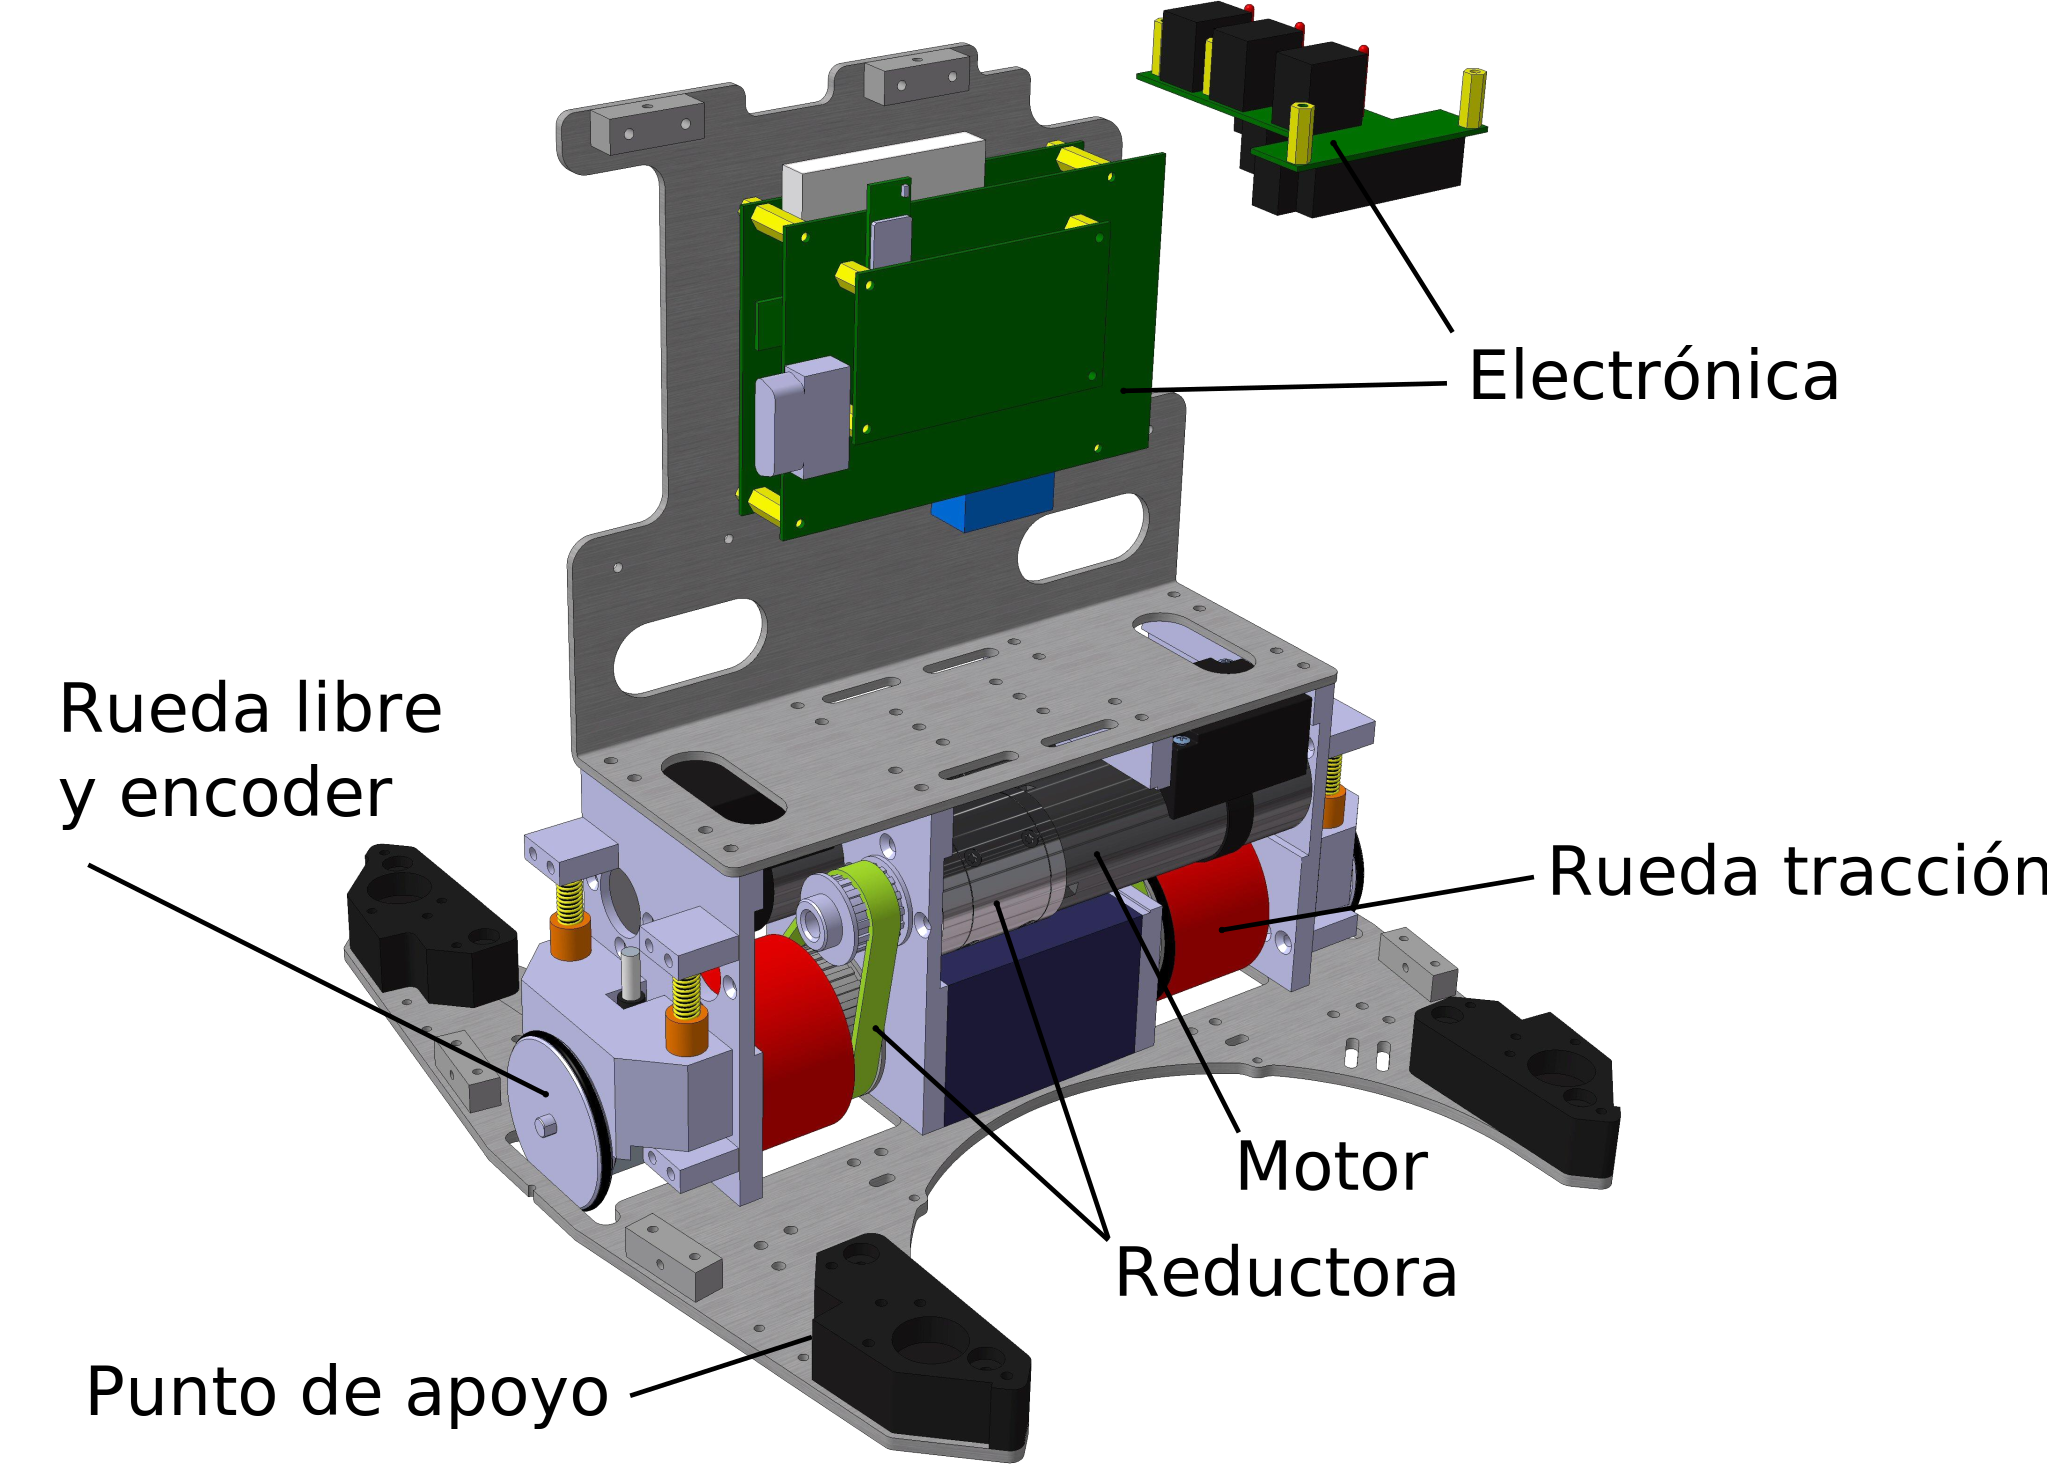
\includegraphics[width=.5\textwidth]{plataforma_partes_1}
\includegraphics[width=.35\textwidth]{plataforma_partes_2}
\caption[]{Elementos de la plataforma rob�tica base}
\label{fig_plataforma_partes_resumen}
\end{figure}

La \textbf{evitaci�n de obst�culos} se realiza a partir de sensores de distancia situados en las caras del robot (ver figura \ref{fig_plataforma_partes_resumen}), y a partir de un \emph{sistema de balizamiento} que hace uso de los soportes y espacios destinados a las balizas de la competici�n Eurobot. �ste sistema, est� compuesto por un sensor tipo faro situado en el robot, y por balizas reflectantes situadas en el oponente (ver figura \ref{fig_plataforma_partes_resumen}). Adem�s, est� espec�ficamente desarrollado para medir la distancia y �ngulo de los oponentes, relativos a la posici�n de la plataforma rob�tica.

% (BALIZA)
El sensor de la baliza tipo faro gira sobre el plano $xy$ y emite una luz que es reflejada por balizas reflectantes, cuando el sensor se encuentra enfrentado con ellas.  La medida de distancia se basa en el principio por el cual, un objeto cercano se ve m�s grande que uno lejano. De forma que, a una distancia cercana le corresponde un �ngulo relativo de detecci�n $\alpha_d$, mayor que el de una distancia m�s lejana. Por otro lado, la medida de �ngulo, se obtiene a partir del �ngulo durante el cual se detecta la baliza reflectante.

% HW
El desarrollo HW presentado, implementa una \textbf{arquitectura HW} que contempla la implementaci�n, tanto de la plataforma rob�tica, como de los sistemas mec�nicos del robot. La arquitectura implementa un sistema embebido basado en microcontroladores dsPIC, que tiene sus recursos repartidos entre la implementaci�n de la plataforma rob�tica y de los sistema mec�nicos. Debido a que los recursos destinados a los sistemas mec�nicos dependen de la tem�tica de la prueba, la arquitectura tiene una interfaz I2C destinada expansi�n de recursos de entrada/salida (E/S) y a la implementaci�n de un procesamiento distribuido.

Por otro lado, la arquitectura HW tiene una interfaz de depuraci�n RS-232 a trav�s de la cual poder controlar, monitorizar y probar el hardware y el software desarrollado. Esta interfaz, forma una cadena serie con el resto de microcontroladores que permite acceder a cualquiera de ellos mediante un \emph{bypass} del los datos. Adem�s, la arquitectura cuenta con una interfaz inal�mbrica Bluetooth, mediante la cual se implementa la \textbf{comunicaci�n con la baliza tipo faro y el robot secundario}. Dependiendo de las caracter�sticas del robot, esta arquitectura HW ha sido implementada en una o varias tarjetas electr�nicas, como se muestra en varios ejemplos de robots desarrollados.


% (ver figura \ref{fig_hardware_arquitectura_principal_resumen}).

%\begin{figure}[ht]
%\centering
%\includegraphics[width=.9\textwidth]{hardware_arquitectura_principal}
%\caption[]{Arquitectura hardware desarrollada}
%\label{fig_hardware_arquitectura_principal_resumen}
%\end{figure}


% SW
Se describe un desarrollo SW que basado en una \textbf{arquitectura SW}, cuya estructura, contempla la implementaci�n funcional de la plataforma rob�tica, los sistemas mec�nicos y las funcionalidades propias de la tem�tica y estrategia de juego del robot de Eurobot. As� mismo, se tratan ejemplos de robots desarrollados que implementan esta arquitectura SW.

La implementaci�n SW de la plataforma rob�tica se ha realizado a partir de las librer�as Aversive \cite{aversive_src}, desarrolladas por el equipo de Eurobot Microb Technology \cite{microb}. Las librer�as Aversive constituyen un marco de trabajo para el desarrollo de sistemas basados en microcontroladores AVR de Atmel. A partir de estas librer�as, se crearon las librer�as Aversive4dspic, una migraci�n de las librer�as Aversive a los microcontroladores dsPIC de Microchip, utilizados por el HW desarrollado. 

La arquitectura SW propuesta se organiza en capas o m�dulos funcionales, de forma que aquellos de nivel superior implementan funciones m�s abstractas que los inferiores. El m�dulo \emph{plataforma rob�tica} incluye las funcionalidades de desplazamiento, localizaci�n y evitaci�n de obst�culos. Al mismo nivel, se encuentra el m�dulo \emph{sistemas mec�nicos}, encargado de controlar los mecanismos utilizados por el robot para manipular los elementos de juego. Ambos m�dulos, se integran y se sincronizan en la capa de \emph{tem�tica de juego}, que implementa las funcionalidades propias de la prueba de Eurobot. El nivel m�s abstracto lo implementa la capa \emph{estrategia de juego}, la cual decide cu�ndo y qu� acciones del juego realizar en cada momento durante un partido de Eurobot.

%\begin{description}
%\item \textbf{Drivers de dispositivos HW}

%Capa de menor nivel que permite abstraer los m�dulos o dispositivos HW del robot, como m�dulos de comunicaci�n del microcontrolador (UART, I2C, SPI, ...) o dispositivos externos a �ste como servomotores, o drivers en puente en H para el control de motores.

%\item \textbf{Plataforma rob�tica base}

%M�dulo que implementa las funcionalidades de la plataforma rob�tica base: control de posici�n, odometr�a, gesti�n de trayectorias y evitaci�n de obst�culos.

%\item \textbf{Sistemas mec�nicos}

%M�dulo que abstrae el control de los diferentes sistemas mec�nicos del robot mediante los cuales se manipulan los elementos del  juego. Este m�dulo a su vez se encuentra dividido en varios niveles, representados en el microcontrolador esclavo del robot principal de la figura \ref{fig_sw_diagrama_bloques_resumen}).

%\item \textbf{Tem�tica de juego}

%Nivel que integra toda la funcionalidad de los niveles inferiores y sistemas externos, como la baliza y el robot secundario, para implementar las funcionalidades del robot relativas a la prueba de Eurobot y a la navegaci�n del robot por el campo de juego.

%\item \textbf{Estrategia de juego}

%Esta capa implementa la estrategia de juego de un partido as� como las diferentes fases de las que se compone un partido.

%\item \textbf{Linea de comandos}

%Capa de mayor nivel que permite ejecutar comandos de cualquier m�dulo o nivel. De esta forma durante el desarrollo de las diferentes capas o m�dulos, las funcionalidades de �stas pueden ser probadas por partes y verificar su correcto funcionamiento.

%\end{description}

%\begin{figure}[t]
%\centering
%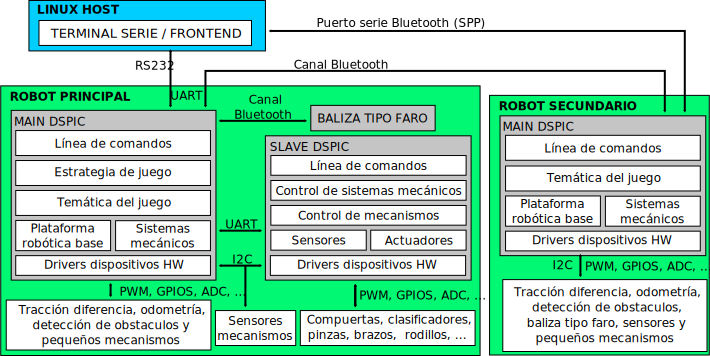
\includegraphics[width=\textwidth]{sw_diagrama_bloques}
%\caption[]{Diagrama de bloques software del robot principal y secundario}
%\label{fig_sw_diagrama_bloques_resumen}
%\end{figure}

%La figura \ref{fig_sw_diagrama_bloques_resumen} representa la implementaci�n de la arquitectura el caso de dos robots: un robot principal y uno secundario se muestra en la figura \ref{fig_sw_diagrama_bloques_resumen}. Ambos robots implementan la misma arquitectura. El robot principal, implementa la arquitectura mediante dos microcontroladores, mientras que el secundario utiliza �nicamente un �nico microcontrolador.

Por �ltimo, el desarrollo SW incluye adem�s un \textbf{simulador de los robots y del campo de juego}. �ste simulador, se implementa a partir de la compilaci�n del c�digo fuente de los robots en un \emph{host} GNU/Linux, y de la emulaci�n del HW y elementos mec�nicos del robot. El entorno de simulaci�n, permite visualizar los movimientos de los robots sobre un campo de juego virtual y simular robots oponentes.






%%% Local Variables:
%%% TeX-master: "../book"
%%% End:


       % EDIT this file

% Now include toc and list of figures+tables
\input{cover/toc+lof+lot.tex}                 % DO NOT TOUCH THIS LINE!

% If you want to include additional listings, you can use the float
% package. As an example, I include here the listing of source code
% snippets (you have some examples in appendix/manual.tex)
\input{cover/extralistings.tex}               % Edit this file or
                                              % comment it out

% Now include acronyms (if this is the case)
\input{acronyms/acronymsgl.tex}               % EDIT this file or
                                              % comment it out if you do
                                              % not use acronyms

% Now include symbols (if this is the case)
\input{symbols/symbolsgl.tex}                 % EDIT this file or
                                              % comment it out if you do
                                              % not use acronyms

%
% END within-document configuration, frontpage and cover pages generation
%%%%%%%%%%%%%%%%%%%%%%%%%%%%%%%%%%%%%%%%%%%%%%%%%%%%%%%%%%%%%%%%%%%%%%%%%%%


%%%%%%%%%%%%%%%%%%%%%%%%%%%%%%%%%%%%%%%%%%%%%%%%%%%%%%%%%%%%%%%%%%%%%%%%%%%
% Now start text and numbering for mainmatter (chapter+appendices)
%%%%%%%%%%%%%%%%%%%%%%%%%%%%%%%%%%%%%%%%%%%%%%%%%%%%%%%%%%%%%%%%%%%%%%%%%%%
\mainmatter                                       % DO NOT TOUCH THIS LINE!
\deactivatetilden                                 % DO NOT TOUCH THIS LINE!


%%%%%%%%%%%%%%%%%%%%%%%%%%%%%%%%%%%%%%%%%%%%%%%%%%%%%%%%%%%%%%%%%%%%%%%%%%%
%%%%%%%%%%%%%%%%%%%%%%%%%%%%%%%%%%%%%%%%%%%%%%%%%%%%%%%%%%%%%%%%%%%%%%%%%%%
%%%%%%%%%%%%%%%%%%%%%%%%%%%%%%%%%%%%%%%%%%%%%%%%%%%%%%%%%%%%%%%%%%%%%%%%%%%
%%%%%%%%%%%%%%%%%%%%%%%%%%%%%%%%%%%%%%%%%%%%%%%%%%%%%%%%%%%%%%%%%%%%%%%%%%%
%%%%%%%%%%%%%%%%%%%%%%%%%%%%%%%%%%%%%%%%%%%%%%%%%%%%%%%%%%%%%%%%%%%%%%%%%%%
%%%%%%%%%%%%%%%%%%%%%%%%%%%%%%%%%%%%%%%%%%%%%%%%%%%%%%%%%%%%%%%%%%%%%%%%%%%
%%%%%%%%%%%%%%%%%%%%%%%%%%%%%%%%%%%%%%%%%%%%%%%%%%%%%%%%%%%%%%%%%%%%%%%%%%%
% BEGIN Normal chapters. Edit/modify all within this section
%
% I don't recommend it, but if you want to define "parts", use this...
% BEWARE: I didn't write the english dependent code
%\part*{Memoria}
%\label{part:memoria}

%%%%%%%%%%%%%%%%%%%%%%%%%%%%%%%%%%%%%%%%%%%%%%%%%%%%%%%%%%%%%%%%%%%%%%%%%%%
%
% Generic template for TFC/TFM/TFG/Tesis
%
% $Id: introduccion.tex,v 1.6 2014/02/11 11:00:06 macias Exp $
%
% By:
%  + Javier Mac�as-Guarasa.
%    Departamento de Electr�nica
%    Universidad de Alcal�
%  + Roberto Barra-Chicote.
%    Departamento de Ingenier�a Electr�nica
%    Universidad Polit�cnica de Madrid
%
% Based on original sources by Roberto Barra, Manuel Oca�a, Jes�s Nuevo,
% Pedro Revenga, Fernando Herr�nz and Noelia Hern�ndez. Thanks a lot to
% all of them, and to the many anonymous contributors found (thanks to
% google) that provided help in setting all this up.
%
% See also the additionalContributors.txt file to check the name of
% additional contributors to this work.
%
% If you think you can add pieces of relevant/useful examples,
% improvements, please contact us at (macias@depeca.uah.es)
%
% Copyleft 2013
%
%%%%%%%%%%%%%%%%%%%%%%%%%%%%%%%%%%%%%%%%%%%%%%%%%%%%%%%%%%%%%%%%%%%%%%%%%%%

\chapter{Introducci�n al proyecto}
\label{cha:introduccion}

\begin{FraseCelebre}
  \begin{Frase}
    Desocupado lector, sin juramento me podr�s creer que quisiera que este
    libro [...] fuera el m�s hermoso, el m�s gallardo y m�s discreto que
    pudiera imaginarse\footnote{Tomado de ejemplos del proyecto \texis{}.}.
  \end{Frase}
  \begin{Fuente}
    Miguel de Cervantes, Don Quijote de la Mancha
  \end{Fuente}
\end{FraseCelebre}


\section{Presentaci�n}
\label{sec:presentacion}

Este trabajo de fin de carrera trata sobre el desarrollo de robots para la competici�n de robots Eurobot \cite{eurobot}. Pretende ser un manual de referencia para todo aquel que quiera construir un robot para participar en Eurobot\footnote{O para desarrollar un robot de similares caracter�sticas para cualquier otro cometido}. Todo lo que se expone en este libro esta se sustenta en la experiencia adquirida en el desarrollo de robots participantes en Eurobot entre los a�os 2003 y 2015. Especialmente en el periodo entre 2010 y 2015.

\section{La competici�n Eurobot}
\label{sec:la_competicion_eurobot}

Eurobot es un concurso internacional de rob�tica creado en 1998 a partir de la Copa de Francia de la rob�tica \cite{cdr} (Coupe de France de robotique). El concurso est� abierto a equipos de j�venes, organizados ya sea en proyectos de estudiantes o en clubes independientes. Eurobot se lleva a cabo en Europa, pero da la bienvenida a los equipos de todos los continentes.

Cada a�o, las reglas se publican alrededor de octubre. Los equipos tienen entonces varios meses para dise�ar y construir sus robots y competir entre abril y junio en el concurso nacional, en el cual se pueden seleccionar s�lo 3 equipos por pa�s. Los mejores equipos de cada pa�s se reunir�n despu�s para competir en las finales de Eurobot.

Las reglas cambian cada a�o, sin embargo, la base es siempre la misma:

\begin{itemize}
\item Los robots tienen aproximadamente el tama�o de un cubo de 30 cm.
\item El campo de juego tiene una dimensi�n de 2 metros de ancho y 3 metros de largo.
\item El juego tiene 90 segundos de duraci�n.
\item Los robots tienen que llevar a cabo varias tareas en el campo con el fin de ganar tantos puntos como sea posible.
\item Los robots tienen que evitarse unos a otros y evitar los choques.
\item Los robots son completamente aut�nomos y deben hacer todas las acciones por ellos mismos.
\end{itemize}

Tal y como est� dise�ado, Eurobot constituye un reto de ingenier�a que permite a alumnos de electr�nica, mec�nica e inform�tica aplicar sus conocimientos o ampliarlos y compartirlos. Tambi�n hace, por ejemplo, que alumnos de electr�nica aprendan mec�nica o inform�tica o ambos campos o todos. Dada la complejidad de los robots suelen ser construidos por equipo formados de al menos 2 personas, lo cual implica cierta organizaci�n, divisi�n de tareas y trabajo en equipo. Un equipo numeroso permite desarrollar robots con partes m�s especializadas pero implica una gesti�n y coordinaci�n mayor. Por otro lado, Eurobot implica confeccionar un producto completo, original y funcional desde cero\footnote{No siempre se ha de empezar desde cero, un desarrollo modular y estructurado permite partir de una base m�nima.} (o como dir�amos en Ingl�s \emph{from scratch}) en cosa de 6 o 7 meses. Esto implica una elecci�n y compra de materiales, componentes, dise�o electr�nico y mec�nico, construcci�n de prototipos, desarrollo de software, ... y en definitiva una gesti�n del tiempo. Tiempo que suele escasear porque los participantes, generalmente alumnos, disponen de �l escasamente\footnote{Y parece ser que menos a�n con los actuales planes de estudios Bolonia}.


La comunidad de Eurobot se comunica principalmente a trav�s de sus foros\cite{foros_eurobot}. Hay tres foros principales: un foro relacionado con las reglas de cada a�o, el foro de Eurobot Open\cite{foro_eurobot_open} y el foro de la Copa de Francia de la rob�tica\cite{foro_copa_francia}. Este �ltimo es el foro m�s activo dado que la Copa nacional de Francia es la de mayor tradici�n y la que re�ne el mayor numero de participantes. Este foro, aunque est� escrito en franc�s, es el que acumula la mayor�a de la informaci�n acerca de la competici�n y de temas t�cnicos. Adem�s, cada equipo suele tener una p�gina web, blog o canal de Youtube donde comparte los avances de los robots que construyen cada a�o.

Eurobot est� organizada gracias la asociaci�n internacional de Eurobot y a la asociaci�n francesa \emph{Planet Sciences}\cite{planet_sciences} y a muchas otras asociaciones, escuelas, universidades y personas voluntarias de los pa�ses participantes. Es incre�ble la cantidad de personas que apoyan Eurobot y trabajan de forma voluntaria sin ninguna remuneraci�n m�s que la satisfacci�n de estar implicados y formar parte de esta fiesta que es Eurobot. Y esto incluye a los participantes, ya que ganar Eurobot no implica ning�n premio econ�mico. En total, un mont�n de gente que trabaja para disfrutar y divertirse con la rob�tica.

\section{El equipo \emph{Eurobotics Engineering}, historia y antecedentes}
\label{sec:equipo_eurobotics}

\emph{Eurobotics Engineering}\cite{arc_robots} es un equipo participante en Eurobot formado por entusiastas de la rob�tica. Est� formado por estudiantes de la Universidad de Alcal� (UAH): ingenieros de telecomunicaci�n, de electr�nica, de telem�tica y de electr�nica industrial.

La historia de este equipo se remonta al a�o 2003, a�o en el que el Departamento de Electr�nica de la UAH decide montar un equipo patrocinado a partir de la iniciativa de un grupo de alumnos de participar en Eurobot 2002. Los integrantes del equipo se renuevan cada a�o excepto algunos que se mantienen. Exceptuando el a�o 2009, el resto de a�os el equipo particip� en Eurobot. En el a�o 2010 Diego Salazar y Javier Bali�as crean el equipo de Eurobot llamado \emph{Eurobotics Engineering} y en el a�o 2011, junto con Nilo Masias, fundaron y la Asociaci�n de Rob�tica de Coslada (ARC).

El equipo Eurobot Engineering particip� en Eurobot desde el a�o 2010 hasta el a�o 2015 (exceptuando el a�o 2013). Durante estos a�os ha contado con el apoyo del Dpto. de Electr�nica de la Universidad de la UAH\cite{depeca,uah} y el Ayuntamiento de Coslada, adem�s del patrocinio de Ayudas Hidr�ulicas\cite{ayudas_hidraulicas}, Carpinter�a Ingl�s, Ro-botica\cite{ro_botica} (2010-2012), el Consejo de estudiantes de la UAH\cite{consejo_de_estudiantes} (2014-2015) y Mobile Minds\cite{mobile_minds} (2015).


\section{La rob�tica educativa}
\label{sec:robotica_educativa}

A d�a de hoy la rob�tica constituye una herramienta educativa muy potente. Permite aprender y poner en practica diferentes ramas de la ciencia. Lo hace a trav�s de la ingenier�a y las �reas de la ciencia en las que se sustenta (matem�ticas, f�sica, qu�mica, entre otras) y utilizando la tecnolog�a actual. Este tipo de educaci�n se denomina STEM\cite{stem} acr�nimo del ingl�s \emph{Science, Technology, Engineering and Mathematics} (Ciencia, Tecnolog�a, Ingenier�a y Matem�ticas). Adem�s permite potenciar la creatividad de las tecnolog�as digitales, m�s all� de la simple explotaci�n de ellas \cite{strategy_1_0}.

Adem�s si la rob�tica se hace en equipo, como suele ser habitual en Eurobot, la rob�tica permite desarrollar habilidades y competencias\cite{robocompetences} como el trabajo en grupo, la motivaci�n personal, gesti�n de retos y objetivo, y el manejo del fracaso y las emociones que implican los errores, entre otras.

Este trabajo de fin de carrera constituye en s� un ejemplo de la rob�tica como herramienta educativa y de sus resultados. Los robots desarrollados ha ayudado adquirir experiencia, conocimientos y experiencias de gran valor a�adido a los estudios universitarios de los diferentes integrantes del equipo \emph{Eurobotics Engineering} y anteriores.

En el campo de la ingenier�a electr�nica y mec�nica, se ha ganado experiencia en el proceso de dise�o, fabricaci�n y montaje de productos que implican una electr�nica y una mec�nica (tarjetas electr�nicas, piezas mec�nicas, mecanismos, cableado, etc). Se han aprendido a trabajar con diferentes tipos de materiales (madera, pl�stico, aluminio, pol�meros, etc), a utilizar herramientas y a fabricar piezas mec�nicas por diferentes procesos de fabricaci�n (impresi�n 3D, fresado, plegado, inyecci�n en silicona, etc.).

El simple hecho de que los robots se muevan y que lo hagan hacia lugares concretos implica la aplicaci�n de las matem�ticas y la f�sica. As�, para ir de un punto $A$ a un punto $B$ se utiliza la trigonometr�a. Esto es, el robot necesita mirar a $B$ (girar un �ngulo $\alpha$) y luego avanzar una distancia $d$. Y adem�s si se desea el tiempo en ir de $A$ a $B$ sea el menor posible es necesario utilizar las leyes de Newton para el calculo de la aceleraci�n y velocidad m�xima, que permitan al robot no derrapar ni pasarse de frenada.

Especialmente, dado que un robot en �ltima medida es controlado desde un microcontrolador o procesador similar, la rob�tica implica adquirir conocimientos sobre la ingenier�a del software y el desarrollo de sistemas embebidos\cite{making_embedded_systems}. Seguramente alg�n momento se quiera utilizar una librer�a o c�digo desarrollada por otras personas pero que resulta muy �til. Se tendr� aque aprender a maneja y confiar en librer�as de terceros y si son de c�digo abierto quiz� permita colaborar y solucionar bugs. Se aprende mucho analizando y comprendiendo el c�digo de otros. Adem�s seguramente estas librer�as utilizar�n alg�n sistema de control de versiones distribuido como Git, Mercurial o centralizado como SVN o incluso sistemas m�s antiguos como CVS. La mayor�a de los desarrolladores de software son reacios al principio a utilizar un sistema de control de versiones, suele ser una decisi�n personal que normalmente cae por su propio peso cuando se trabaja con proyectos de c�digo extensos.

A medida que el c�digo desarrollado vaya creciendo surgen planteamientos de como organizarlo, como reutilizar c�digo de un a�o a otro o incluso como reutilizar c�digo del microcontrolador que se est� utilizando para poder utilizarlo en otros proyectos. Esto lleva a desarrollar c�digo de una forma m�s modular y estratificada. Quiz� m�s adelante, el microcontrolador utilizado hasta el momento se quede escaso de recursos, se quiera cambiar a otro de la misma familia pero con m�s recursos y reutilizar las librer�as que se han desarrollado hasta entonces y mantener la compatibilidad con el antiguo microcontrolador. Esto por ejemplo se puede lograr mediante la compilaci�n condicional.

Al ir ganando experiencia, se es capaz de detectar las partes fundamentales y comunes a la hora de implementar una aplicaci�n o funcionalidad. Si se observa como lo ha resuelto el resto del mundo se cae en la cuenta que hay ciertas cosas que ya est�n muy estudiadas y aparecen en cualquier aplicaci�n que desarrollemos. As� se podr� detectar y aplicar patrones que facilitan desarrollo.

Quiz� llegue un momento en que el tiempo que lleva realizar la depuraci�n del robot sobre el entorno real es mucho y es un proceso lento, o quiz� no se disponga de dicho entorno porque no queda otra opci�n que desarrollar de forma remota. Para todo eso, es muy �til el uso de simuladores o bancos de pruebas\footnote{Tambi�n conocidos en la literatura anglosajona como \emph{sandbox}.} que permiten emular las interfaces de entrada y salida del robot (sensores y motores) o sus est�mulos (obst�culos).

La rob�tica se disfruta, es divertida, pero tambi�n se sufre y requiere de un indudable ejercicio de abstracci�n y concentraci�n. Es necesario investigar sobre cosas nueva o reforzar conocimientos ya adquiridos, aplicarlos y madurarlos. Son m�s comunes los errores que los aciertos, nada sale a la primera, y la \emph{ley de Murphy}\footnote{"Si algo puede salir mal, saldr� mal"} suele no fallar.  Todo esto lleva al aprendizaje y aplicaci�n del \emph{m�todo cient�fico} para experimentar o para resolver problemas encontrados, como comportamientos no esperados del robot.

Durante el desarrollo de la rob�tica, puede parecer que es una actividad poco agradecida o agradecida en momentos muy cortos. Pero merece la pena y adem�s se demuestra que m�s tarde, en el mundo laboral o de la investigaci�n, es cuando la rob�tica tiene gran parte su retorno\footnote{El autor de este proyecto esta convencido de ello y lo ha experimentado.}.


\section{Aprendiendo de gigantes.}
\label{sec:aprendiendo_de_gigantes}

Hoy en d�a es casi impensable que una sola persona pueda realizar avances en los diferentes campos de la ciencia equiparables a los descubrimientos de los grandes cient�ficos de la historia. As� la investigaci�n y el desarrollo tecnol�gico son llevados a cabo por grupos de personas cada cual experta en ciertos tema concretos. Por otro lado la tecnolog�a y sus aplicaciones cada vez son m�s complejas y eso es en gran parte a que los nuevos desarrollos se apoyan en desarrollos anteriores que permiten abstraerse de aquello que se encuentra fuera del alcance de un objetivo concreto.

Quiz� el ejemplo m�s conocido a d�a de hoy es la plataforma de desarrollo Arduino\cite{arduino} que permite desarrollar sistemas embebidos partiendo de un conocimiento muy b�sico o nulo sobre microcontroladores. Esto es gracias a que la plataforma de desarrollo Arduino tiene una vasta librer�a de funciones que abstraen la programaci�n de bajo nivel del microcontrolador de forma que no se \emph{escribe un bit} de uno o varios \emph{registros} de nombres aparentemente sin significado, si no que se \emph{detiene}, se \emph{cambia el sentido} o se \emph{cambia la velocidad} de un \emph{motor}. Adem�s todas esas funciones se encuentran documentadas y son accesibles\cite{arduino_src} para su modificaci�n o consulta. As�, si una funcionalidad de una librer�a no existe, es posible estudiar como est� implementada y a�adir nuevas funcionalidades.

En cierta forma, esta manera de abordar el aprendizaje y el desarrollo de aplicaciones tecnol�gicas es una forma natural y acorde con el desarrollo tecnol�gico de la sociedad actual. Hoy en d�a la tecnolog�a que utilizamos en el d�a a d�a es compleja y muy abstracta por lo que no tiene sentido que el aprendizaje de la misma comience desde los niveles m�s b�sicos. Plataformas como Arduino permiten comenzar en un punto intermedio y poder crecer hacia niveles de abstracci�n mayores (grano grueso) o hacia niveles inferiores m�s espec�ficos (grano fino).

Pues bien este proyecto no es una excepci�n y tambi�n se ha apoyado en hombros de gigantes. El c�digo fuente de los microcontroladores de algunos de los robots desarrollados (Husillo, Joselito o Campanolo) fue escrito desde cero. Otros (Electrococo, Mr.Proper y Topolino) se ayudaron del c�digo escrito en a�os anteriores para para otros robots. Y finalmente a partir del a�o 2010 los robots (Trompetero, Zamorano, Autom�tico, Crispin, P.Tinto y Tirantes) se desarrollaron a partir del c�digo abierto escrito por terceros.

El utilizar c�digo abierto de terceros vino dado por el objetivo de evolucionar tecnol�gicamente los robots a desarrollar para Eurobot. Para ello se estudi� los fundamentos t�cnicos y tecnol�gicos de los robots por aquella �poca obten�an muy buenos resultados como RCVA\cite{rcva}, Microb Tecnology\cite{microb}, RCA Archen\cite{rca_aachen} o Turak\cite{turak}. Al final de dicho estudio se establecieron los requisitos de la mec�nica, hardware y software necesarios, y se desarrollo una plataforma rob�tica base (el \emph{Dummy robot}, ver \ref{dummy_robot}) con una mec�nica y una electr�nica de acuerdo a los requisitos buscados.

\begin{figure}
\centering
\includegraphics[height=.2\textheight]{dummy_robot_1}
\hspace{1cm}
\includegraphics[height=.2\textheight]{dummy_robot_2}

\caption{\emph{Dummy robot}. Plataforma rob�tica base desarrollada en 2010. Dise�o mec�nico: Diego Salazar Accuci. Electr�nica y programaci�n: Javier Balinas.}

\label{dummy_robot}
\end{figure}


Al final del proceso de estudio se descubrieron las librer�as Aversive desarrolladas por el equipo \emph{Microb Technology} para microcontroladores AVR de Atmel. Por aqu�l entonces, la electr�nica que se estaba dise�ando estaba basada en microcontrolador dsPIC de Microchip. Podr�amos a ver migrado el HW y utilizar microcontroladores AVR, pero al final se opt� por migrar las librer�as Aversive a la arquitectura de dsPIC, lo que se denomin� Aversive4dsPIC\footnote{Pronunciado \emph{Aversive for dsPIC}, Aversive para dsPIC}.

La decisi�n de utilizar estas librer�as y portarlas permiti� no solo aprender a utilizarlas desde la capa de aplicaci�n (el robot) sin no estudiar como estaban implementadas y adaptarlas para ser compatibles con una arquitectura diferente. En definitiva se reutiliz� el c�digo de terceros, lo cual implica mucho m�s que el simple hecho de aprovechar el trabajo realizado por otros. En este caso las librer�as Aversive\cite{aversive_src} son unas librer�as libres desarrolladas por varias personas, versionada bajo un sistemas de control de versiones, que est�n muy bien estructuradas, escritas siguiendo una gu�a de estilo com�n, que explota al m�ximo el lenguaje ANSI C, que cuenta con un \emph{toolchain}\footnote{Cadena de herramientas: conjunto de programas mediante los cuales se construye el programa que se ejecuta en el microcontrolador} que utiliza herramientas libres, que implementan todo tipo de funcionalidades y muchas de ellas dirigidas al desarrollo de robots como los de Eurobot. La migraci�n de las librer�as Aversive se realiz� siguiendo y manteniendo toda las caracter�sticas anteriormente mencionada, lo cual implic� el aprendizaje de las mismas y de todos los conceptos derivados y subyacentes de ellas.     



\section{Motivaci�n y objetivos}
\label{sec:motivacion_y_objetivos}

Todo el trabajo realizado en el desarrollo de los diferentes robots viene principalmente motivado por la afici�n a la rob�tica, la electr�nica, los sistemas embebidos y por la inquietud de inventar y crear cosas.

Por otro lado, el objetivo fundamental de este trabajo es la divulgaci�n del conocimiento adquirido en la realizaci�n de robots que compiten en Eurobot, siendo los objetivos espec�ficos de este proyecto los siguientes:

\begin{itemize}
\item Reflexionar y analizar diferentes aspectos indirectamente relacionados con el desarrollo de ingenier�a (el equipo de trabajo, organizaci�n, ...)
\item Analizar y describir los fundamentos de ingenier�a impl�citos (din�mica, cinem�tica, sistemas de control, ...).
\item Describir las partes fundamentales del desarrollo (movimiento, navegaci�n, posicionamiento, estrategia ...) y dise�o un robot de Eurobot (mec�nica, electr�nica, programaci�n, ...).
\item Presentar implementaciones y dise�os reales de cada una de las partes fundamentales de un robot de Eurobot.
\item Documentar todas aquellos dise�os, desarrollos o algoritmos realizados que puedan servir de punto de partida o ser reutilizados en futuros desarrollos (dise�os electr�nicos, librer�as software, herramientas de simulaci�n, ...).
\end{itemize}

\section{Organizaci�n del libro}
\label{sec:organizacion_del_libro}

El libro cuenta con 5 cap�tulos adicionales a este cap�tulo:

\begin{description}

\item El robot de Eurobot

Cap�tulo que describe las partes o fases principales implicadas en el desarrollo de un robot de Eurobot: las especificaciones funcionales (las reglas del juego), las partes principales de un robot de Eurobot, las caracter�sticas de la mec�nica, electr�nica y software, las fases t�picas de dise�o y la depuraci�n y puesta en marcha del robot.

\item El equipo de Eurobot

Reflexi�n sobre el equipo de personas que desarrollan un robot de Eurobot y varios temas relacionados como el n�mero de integrantes, expectativas, motivaci�n y objetivos del equipo, divisi�n de tareas o la organizaci�n y metodolog�a de trabajo.

\item Plataforma rob�tica base

Descripci�n de lo que se ha considerado plataforma rob�tica base, un robot base cuyas caracter�sticas y funcionalidades son comunes a cualquier juego de Eurobot y sobre el que desarrollar nuevos robots participantes. El cap�tulo se centra en un robot de tracci�n diferencial y control de posici�n polar mediante odometr�a. Adem�s trata el sistema desarrollado para la detecci�n y evitaci�n de los robots oponentes.

\item Sistemas mec�nicos para la manipulaci�n de elementos de juego

Cap�tulo que trata sobre los sistemas mec�nicos (brazos, pinzas, catapultas, etc.) que se desarrollan espec�ficamente para manipular los elementos de juego de la prueba de Eurobot. Se realiza una revisi�n de las soluciones mec�nicas conocidas y utilizadas hasta la fecha por diferentes equipos. Y posteriormente se tratan los componentes fundamentales de estos sistemas mec�nicos (actuadores y sensores) y la forma de controlarlos y sincronizarlos con el movimiento del robot.  

\item Implementaci�n de la estrategia de juego

Por �ltimo se trata el tema de la estrategia de juego de un robot de Eurobot. Se analiza los elementos y diferentes fases en las que se puede dividir un partido y los diferentes patrones de implementaci�n software. Se trata la gesti�n de trayectorias durante un partido, algo nada determinista dado que se compite con un oponente del que se desconoce el comportamiento. Adem�s tambi�n se habla de las estrategias con dos robots y sobre la simulaci�n de las estrategias y sus ventajas. 

\end{description}



%%% Local Variables:
%%% TeX-master: "../book"
%%% End:


%%%%%%%%%%%%%%%%%%%%%%%%%%%%%%%%%%%%%%%%%%%%%%%%%%%%%%%%%%%%%%%%%%%%%%%%%%%
%
% Generic template for TFC/TFM/TFG/Tesis
%
% $Id: introduccion.tex,v 1.6 2014/02/11 11:00:06 macias Exp $
%
% By:
%  + Javier Mac�as-Guarasa.
%    Departamento de Electr�nica
%    Universidad de Alcal�
%  + Roberto Barra-Chicote.
%    Departamento de Ingenier�a Electr�nica
%    Universidad Polit�cnica de Madrid
%
% Based on original sources by Roberto Barra, Manuel Oca�a, Jes�s Nuevo,
% Pedro Revenga, Fernando Herr�nz and Noelia Hern�ndez. Thanks a lot to
% all of them, and to the many anonymous contributors found (thanks to
% google) that provided help in setting all this up.
%
% See also the additionalContributors.txt file to check the name of
% additional contributors to this work.
%
% If you think you can add pieces of relevant/useful examples,
% improvements, please contact us at (macias@depeca.uah.es)
%
% Copyleft 2013
%
%%%%%%%%%%%%%%%%%%%%%%%%%%%%%%%%%%%%%%%%%%%%%%%%%%%%%%%%%%%%%%%%%%%%%%%%%%%

\chapter{El robot de Eurobot}
\label{cha:el_robot_de_eurobot}

\begin{FraseCelebre}
  \begin{Frase}
    Desocupado lector, sin juramento me podr�s creer que quisiera que este
    libro [...] fuera el m�s hermoso, el m�s gallardo y m�s discreto que
    pudiera imaginarse\footnote{Tomado de ejemplos del proyecto \texis{}.}.
  \end{Frase}
  \begin{Fuente}
    Miguel de Cervantes, Don Quijote de la Mancha
  \end{Fuente}
\end{FraseCelebre}



\section{Introducci�n}

Cada robot que participa en Eurobot es �nico y diferente al resto, sin embargo todos tienen en com�n ciertas caracter�sticas o funcionalidades que vienen determinadas o derivadas de las reglas del juego. Como se ha comentado en el capitulo \ref{cha:introduccion} cada a�o la prueba en la que competir o a resolver es diferente, esto tiene una implicaci�n directa en el dise�o mec�nico especialmente en los mecanismos dise�ados para manipular los elementos de juego propios de la prueba. Sin embargo, si se comparan las reglas del juego de varios a�os se observan caracter�sticas comunes que repercuten en el dise�o de la mec�nica, de la electr�nica o del software.

\section{Especificaciones del robot de Eurobot}
\label{sec:especificaciones_del_robot_de_eurobot}

Un robot de Eurobot tiene especificaciones independientes de la tem�tica del juego y otras dependientes totalmente. Las primera permiten que una vez est�n desarrolladas y validadas puedan ser reutilizadas o mejoradas en futuros dise�os. Esto quiere decir que pueden ser un bloque totalmente modular, por ejemplo una tarjeta electr�nica, o dise�os reutilizables como el dise�o electr�nico de la tarjeta, cuyo PCB\footnote{Del ingl�s \emph{Printed Circuit Board}, Tarjeta de Circuito Impreso} puede dise�arse a medida del robot y en funci�n del espacio disponible.

Por otro lado, los sistemas mec�nicos a dise�ar para la manipulaci�n de los elementos de juego son en su mayor�a espec�ficos de cada prueba. S�lo una peque�a parte del desarrollo relacionado con estos sistemas es reutilizable, como es parte del desarrollo software destinado al control de dichos sistemas mec�nicos. 

Un robot de Eurobot ha de ser completamente aut�nomo y b�sicamente ser capaz de:

\begin{enumerate}
\item Desplazarse hasta las diferentes zonas del campo donde se sit�an los elementos del juego o donde se almacenan.
\item Evitar chocar con elementos del campo de juego y con otros robots oponentes durante los desplazamientos entre zonas del campo.
\end{enumerate}

Adem�s, si las reglas permiten dos robots por equipo: un robot principal y uno secundario, es recomendable que ambos robots sean capaces de comunicarse entre s� con el fin jugar de forma cooperativa.

Con el fin de facilitar la detecci�n entre los robots y que estos sean capaces de evitar colisiones entre ellos, los robots han de reservar un espacio para sensores y balizas a una altura determinada como muestra la figura \ref{fig:balizas_robots}. As�, cada robot puede colocar una baliza o marca en el robot oponente y disponer de un espacio donde situar los sensores apropiados para detectar dicha baliza. 

Estas balizas pueden ser activas o pasivas. Por ejemplo, un sistema compuesto por una baliza maciza y un sensor de ultrasonidos puede ser utilizado para detectar a que distancia y direcci�n se encuentra un robot oponente antes de tomar tomar la decisi�n de hacia donde redirigirse.

Adem�s el campo de juego cuenta con 3 soportes para balizas adicionales que est�n a disposici�n de cada equipo (ver figura \ref{fig:balizas_campo}). Estos soportes est�n pensados para facilitar la localizaci�n de los robots en el campo de juego. Por ejemplo, un sistema compuesto por una baliza reflectante colocada en el soporte de una esquina del campo y un sensor de luz reflexivo en el robot puede ser utilizado para localizar una canasta que se encuentre en dicha esquina del campo.

Las balizas pueden ser activas o pasivas y tiene como �nicas restricciones sus dimensiones y peso:

\begin{itemize}
\item Balizas colocadas en el oponente: dimensiones m�ximas de 80x80x80 cm y peso m�ximo de 0,5 Kg.
\item Balizas del campo de juego: dimensiones m�ximas de 160x80x80 cm.
\item Espacio para sensores en cada robot: 80x80x80 cm. 
\end{itemize}

\begin{figure}[ht]
\centering
\includegraphics[height=.27\textheight]{balizas_robots}
\caption{Altura de balizas y sensores. Vista de perfil de dos robots oponentes y el campo de juego. 1- Soporte para balizas del campo de juego. 2- Soporte para baliza del oponente. 3- Espacio para sensores de balizas.}
\label{fig:balizas_robots}
\end{figure}

\begin{figure}[ht]
\centering
\includegraphics[height=.27\textheight]{balizas_campo}
\caption{Campo de juego de Eurobot 2015. Soportes para balizas fijas de los equipos A y B.}
\label{fig:balizas_campo}
\end{figure}

Por otro lado, el robot ha de ser capaz de resolver la tem�tica del juego lo cual implica el manejo de los elementos o piezas propias del juego. Por ejemplo, en Eurobot 2015, juego titulado como \emph{Robomovies} (tem�tica sobre el cine), una de las cosas por las que los robots obten�an puntos era por hacer una torre con piezas cil�ndricas coronada con una pelota de tenis que simbolizaba un foco de cine. 

Adem�s, mec�nicamente un robot ha de cumplir las siguientes restricciones dimensionales:

\begin{itemize}
\item Per�metro m�ximo inicial 1200 mm (700 mm para el robot secundario)
\item Per�metro m�ximo desplegado 1500 mm (900 mm para el robot secundario)
\item Altura m�xima de 350 mm
\end{itemize}


Por �ltimo, las reglas de Eurobot adem�s especifican otros temas que deben de ser tenidos en cuenta en caso de que apliquen:

\begin{itemize}
\item Fuentes de alimentaci�n y bater�as
\item Utilizaci�n de fuentes de luz y l�seres
\item Utilizaci�n de sistemas de comunicaci�n de radio
\item Utilizaci�n de sistemas de aire comprimido
\item Bot�n de parada de emergencia
\item M�todo de comienzo y finalizaci�n de un partido
\item Procedimientos de un partido.
\end{itemize}


\section{Partes principales en el desarrollo de un robot de Eurobot}

Teniendo en cuenta las especificaciones descritas en la secci�n anterior y la tem�tica de la prueba de Eurobot, el desarrollo de un robot de Eurobot se puede dividir en las siguientes partes principales:

\begin{enumerate}
\item Estrategia de juego.
\item Desplazamiento y localizaci�n.
\item Evitaci�n de obst�culos.
\item Comunicaci�n entre robots (en caso de jugar con 2 robots).
\item Manipulaci�n de elementos de juego. 
\end{enumerate}

As�, tal y como representa la figura \ref{fig:partes_robot_eurobot}, un �nico robot est� compuesto por las tres primera partes y s�lo en caso de contar con 2 o m�s robots es necesaria la parte de comunicaci�n entre robots. 

\begin{figure}[h]
\centering
\includegraphics[height=.4\textheight]{partes_robot_eurobot}
\caption{Partes principales del desarrollo de un robot de Eurobot. En el fondo robot P.Tinto y Tirantes (robot secundario) desarrollados para Eurobot 2015 por el equipo Eurobotics Engineering}
\label{fig:partes_robot_eurobot}
\end{figure}

Por otro lado, las partes 2, 3 y 4 forman lo que se ha denominado \emph{plataforma rob�tica base}. Esta plataforma base est� compuesta por las partes que permiten un desarrollo independientemente de la tem�tica de la prueba de Eurobot. As�, esta plataforma rob�tica constituye un desarrollo reutilizable en la concepci�n de nuevos robots de Eurobot. 

Cada una de estas partes principales de un robot de Eurobot tienen pueden implicar un desarrollo mec�nico, electr�nico y de software, dependiendo del caso.


\subsection{Estrategia de juego}
\label{sec:estrategia_de_juego}

La estrategia de juego constituye el nivel m�s abstracto del robot y tiene un desarrollo puramente software. La estrategia tiene en cuenta diferentes variables del juego como se indica en la figura \ref{fig:variables_estrategia}(tareas por realizar, prioridad de tareas, posici�n del oponente, el tiempo transcurrido de partido, etc.) para tomar decisiones que maximicen la puntuaci�n a conseguir y as� ganar el partido.

\begin{figure}[h]
\centering
\includegraphics[width=.8\textwidth]{variables_estrategia}
\caption{Estrategia de juego: variables a tener en cuenta en la toma de decisiones.}
\label{fig:variables_estrategia}
\end{figure}

El desarrollo de la estrategia puede ser realizado en paralelo a otras partes del robot, pero ha de tener en cuenta los tiempos derivados de tareas que impliquen sistemas mec�nicos, como por ejemplo coger una pelota y almacenarla o desplazarse de un punto del campo a otro. Dichos tiempos por lo general son mucho mayores (segundos o decenas de segundos) que el tiempo que tarda el algoritmo de estrategia implementado en tomar una decisi�n. Es por ello que dicho algoritmo estar� la mayor parte del tiempo esperando a que otras partes terminen de realizar su funci�n.

\subsection{Desplazamiento y localizaci�n}
\label{sec:desplazamiento_y_localizacion}

Un robot de Eurobot est� dise�ado para funcionar en un entorno de dimensiones conocidas como es el campo de juego (un �rea de 2x3 m), o lo que es lo mismo un plano cartesiano. As� la posici�n del robot y otros objetos del campo, como elementos de juego o los robots oponentes, vendr� dada por sus coordenadas rectangulares $(x,y)$ y polares $(d,a)$ relativas a un origen de coordenadas $(0,0)$ (ver figura \ref{fig:ejemplo_campo_cartesiano_y_trayectorias}).

La localizaci�n permite al robot conocer su posici�n $(x_R,y_R)$ en el campo y poder calcular las distancias (rectangulares o polares) de un punto de destino $(x_i,y_i)$ relativas a su posici�n. El desplazamiento permite recorrer dichas distancias a una velocidad $v$ y aceleraci�n $a$ determinadas generando as� \emph{trayectorias}.

\begin{figure}[h]
\centering
\includegraphics[height=.4\textheight]{ejemplo_campo_cartesiano_y_trayectorias}
\caption{Representaci�n cartesiana del campo de Eurobot 2015 (ver figura \ref{fig:ejemplo_campo_cartesiano_y_trayectorias}) y ejemplo de generaci�n de trayectorias. En horizontal el eje $x[mm]$, vertical el eje $y[mm]$. Los cuadrados rojos representan obst�culos y el cuadrado azul de rayas la zona �til de desplazamiento del robot. El punto azul grande con flecha indica la posici�n de inicio y los puntos azules grandes sin flecha indican un punto de destino. Los puntos azules peque�os indican puntos de la trayectoria.}
\label{fig:ejemplo_campo_cartesiano_y_trayectorias}
\end{figure}

Mec�nicamente es necesario desarrollar un sistema de tracci�n, que en el caso de los robots desarrollados es un \emph{sistema de tracci�n diferencial}. Dicho sistema est� compuesto por dos motores con reductora que mueven dos ruedas independientes que est�n en contacto con el campo de juego. Adem�s para poder \emph{controlar velocidad y aceleraci�n} de cada rueda se utilizan sensores tipo \emph{encoder} que miden cuanto gira cada rueda, o lo que es lo mismo su posici�n angular relativa. Utilizando la informaci�n medida por los encoders (u otro sistema similar) es posible medir la posici�n del robot de forma relativa a una posici�n de inicio mediante \emph{algoritmos de odometr�a}\footnote{De forma complementaria se pueden utilizar sistemas de medida de posici�n absoluta para corregir los errores de las medidas relativas}.

Como muestra la figura \ref{fig:desplazamiento_y_localizacion_bloques} la electr�nica asociada ha de contar con una etapa de electr�nica de potencia que permita la excitaci�n de los motores (\emph{drivers} de motores), el acondicionamiento y decodificaci�n de las se�ales de los encoders, y un microcontrolador donde se implementen los algoritmos de control de posici�n, velocidad y aceleraci�n de los motores, y el algoritmo de odometr�a.

\begin{figure}[h]
\centering
\includegraphics[width=.8\textwidth]{desplazamiento_y_localizacion_bloques}
\caption{Desplazamiento y localizaci�n: diagrama de bloques del desarrollo mec�nico, electr�nico y software implicado.}
\label{fig:desplazamiento_y_localizacion_bloques}
\end{figure}

Dicho microcontrolador, adem�s de implementar los algoritmos espec�ficos de control de motores y odometr�a, ha de implementar funciones mucho m�s abstractas como la \emph{generaci�n de trayectorias}. De forma que en �ltima medida, el robot pueda desplazarse a un punto del campo de juego de forma aut�noma o seguir un camino compuesto por varios puntos como el representado en la figura \ref{fig:ejemplo_campo_cartesiano_y_trayectorias}.

\subsection{Evitaci�n de obst�culos}
\label{sec:evitacion_de_obstaculos}

El robot de Eurobot se encuentra con dos tipos de obst�culos a evitar en sus trayectorias. Por un lado est�n los obst�culos fijos y de posici�n conocida como pueden ser partes del campo de juego o elementos de juego al inicio del partido. Y por otro lado, objetos de posici�n desconocida como son los robots oponentes o elementos de juego que han sido movidos de su posici�n inicial.

La evitaci�n de obst�culos est� directamente relacionada con la generaci�n de trayectorias del robot, teni�ndose en cuenta previamente al calculo de la trayectoria a realizar y durante la misma. Los sistemas de detecci�n de obst�culos a desarrollar dependen de las diferente situaciones que se dan en un partido de Eurobot:

\begin{description}
\item \textbf{Objetos en trayectorias de un punto a otro del campo}

Es el caso en el que el robot quiere ir de una zona del campo a otra, por ejemplo para coger o dejar un elemento de juego. El camino a seguir hasta la zona de destino ha de tener en cuenta los espacios libres del campo de juego y la posici�n de los robots oponentes para as� seguir trayectorias libres de obst�culos. Como muestra el ejemplo de la figura \ref{ejemplo_trayectorias_y_evitacion}, entre el punto origen y destino adem�s de los objetos fijos del campo de juego se encuentra el robot oponente. La generaci�n de trayectorias tiene en cuenta estos obst�culos y genera trayectorias que rodean los obst�culos siguiendo el camino m�s corto.


\begin{figure}[h]
\centering
\includegraphics[width=.8\textwidth]{ejemplo_trayectorias_y_evitacion}
\caption{Evitaci�n de obst�culos en trayectorias de una zona a otra del campo. En el centro un robot oponente. En horizontal el eje $x[mm]$, vertical el eje $y[mm]$. Los cuadrados rojos representan obst�culos y el cuadrado azul de rayas la zona �til de desplazamiento del robot. El punto azul grande con flecha indica la posici�n de inicio y los puntos azules grandes sin flecha indican un punto de destino. Los puntos azules peque�os indican puntos de la trayectoria.}
\label{fig:ejemplo_trayectorias_y_evitacion}
\end{figure}


La evitaci�n los obst�culo fijos del campo de juego se puede realizar utilizando la \emph{localizaci�n del robot}. Si el robot conoce su posici�n es sencillo evitar chocar con paredes o elementos fijos del campo de juego.

Respecto a la evitaci�n y detecci�n de los robots oponentes es necesario desarrollar un sistema espec�fico para ello. Este sistema normalmente utiliza los soportes de balizas especificado por las reglas de Eurobot (ver figura \ref{sec:especificaciones_del_robot_de_eurobot}). Dependiendo del sistema de balizas utilizado\ref{balizas_y_cerveza} el desarrollo del mismo implicar� en mayor o mejor medida un desarrollo mec�nico, electr�nico o software. 

Sea cual sea el sistema utilizado para localizar al robot oponente, debe de aportar la informaci�n de la posici�n del �ste de forma relativa a la posici�n del robot (ver ejemplo de la figura \ref{fig:medida_posicion_oponente} o absoluta respecto al origen de coordenadas del campo de juego. Adem�s otras caracter�sticas deseables son un rango de detecci�n que cubra todo el campo de juego y un tiempo de medici�n de la posici�n del oponente peque�o. El conocer en todo momento la posici�n del oponente constituye una informaci�n muy valiosa a tener en cuenta en la estrategia de juego. As� mismo, un tiempo de medici�n peque�o permitir� un menor tiempo de reacci�n en caso de peligro de colisi�n.

\begin{figure}[h]
\centering
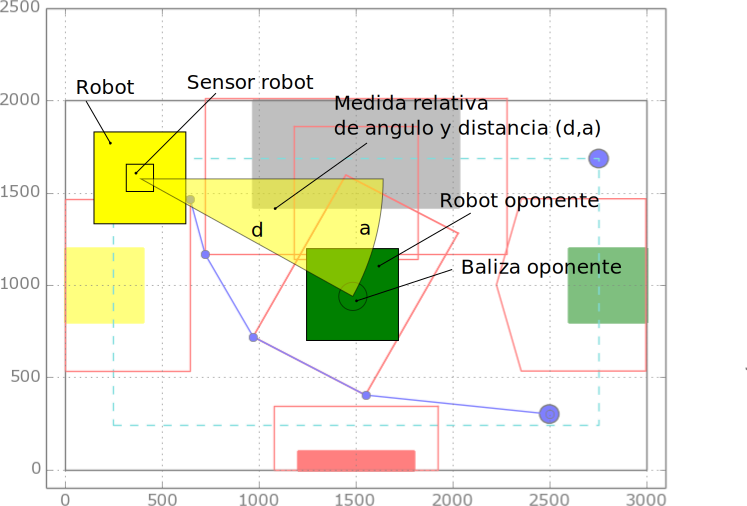
\includegraphics[width=.8\textwidth]{medida_posicion_oponente}
\caption{Ejemplo de sistema de medida de la posici�n del robot oponente que utiliza una baliza colocada en el oponente y un sensor en el robot. La medida obtenida es el �ngulo y la distancia relativa al la posici�n del robot.}
\label{fig:medida_posicion_oponente}
\end{figure}


\item \textbf{Objeto inesperado en una trayectoria}

Iniciada una trayectoria, que a priori no tiene obst�culos, en cualquier punto de esta puede ocurrir que el robot oponente cambie su posici�n y se interponga en el camino del robot pudiendo producirse una colisi�n. En este caso, el robot ha de detectar este obst�culo inesperado y parar o modificar su trayectoria para evitar la colisi�n.

La detecci�n de un objeto inesperado en una trayectoria se puede realizar utilizando el mismo sistema desarrollado para localizar al robot oponente, si el rango de medida cubre distancias cercanas al robot y el tiempo de medida es suficientemente peque�o respecto a la velocidad de desplazamiento del robot. A�n as�, un segundo sistema m�s especifico para estos casos aumenta la fiabilidad y permite hacer una doble comprobaci�n si los rangos de detecci�n de ambos sistemas se solapan.

El sistema a desarrollar permite detectar un objeto cercano (0 a 30cm aproximadamente) en las direcci�n de avance del robot (parte delantera y trasera) y opcionalmente detectar un objeto situado a los lados del robot (lado izquierdo y derecho). El rango depende de principalmente de la distancia de frenado del robot a velocidad m�xima, de forma que la detecci�n de un objeto permita evitar la colisi�n. 

Suelen utilizarse sensores digitales de luz difusa (luz roja o infrarrojos) situados estrat�gicamente a una altura determinada. En parte delantera y trasera del robot tres sensores son suficientes para detectar un objeto (dos si el robot es estrecho), dos de ellos se sit�an en los extremos de del robot y si fuera necesario un tercero en el punto medio entre ellos (ver figura \ref{fig:deteccion_obstaculo_en_trayectoria}). Para la detecci�n de objetos a izquierda y derecha del robot un sensor a cada lado es suficiente. El fundamento es simple, si cualquiera de los dos sensores de los extremos de robot detecta un objeto hay posibilidad de colisi�n.

\begin{figure}[h]
\centering
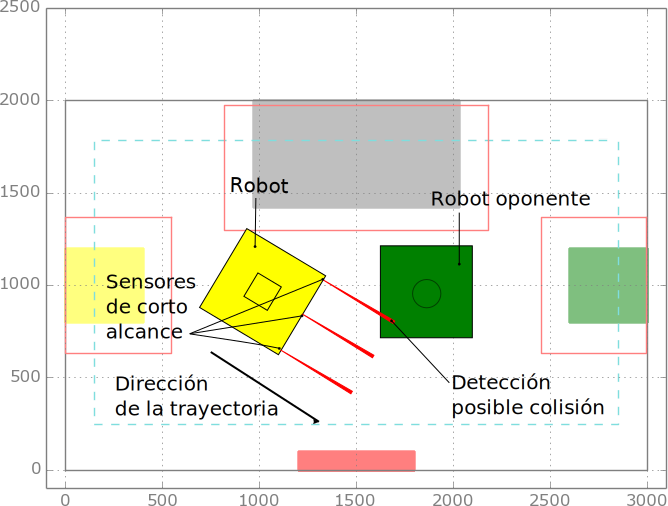
\includegraphics[width=.8\textwidth]{deteccion_obstaculo_en_trayectoria}
\caption{Ejemplo de sistema de detecci�n de obst�culos en trayectoria. Tres sensores de corta distancia digitales detectan posibles colisiones.}
\label{fig:deteccion_obstaculo_en_trayectoria}
\end{figure}


\item \textbf{Objeto que bloquea un elemento del juego}

Caso en el que el robot se encuentra en una zona desde donde necesita acceder a un elemento de juego, por ejemplo un dispensador de fichas. Puede ocurrir que uno de los elementos de juego, por ejemplo una pelota u otro elemento, se encuentre entre el robot y el dicho dispensador. La probabilidad de que ocurra esto es mayor con los objetos esf�ricos y de poco peso, como por ejemplo pelotas de \emph{ping pong}, la manipulaci�n de los mismos puede hacer que �stos rueden a lo largo del campo aleatoriamente con facilidad\footnote{Este tipo de objetos tambi�n puede entrar dentro de los sistemas mec�nicos del robot e inutil�zalos o bloquearlos}. 

Otro caso, que se suele dar muy pocas veces, es que el robot oponente est� protegiendo un elemento de juego com�n de forma premeditada utilizando otro elemento de juego, con el fin de dificultar su acceso al otro robot.

En el caso de que un objeto se encuentre entre un elemento fijo del campo, como una pared, y el robot. Si el robot necesita utilizar dicha pared como referencia y un objeto se encuentra en medio, la referencia que medir� el robot ser� err�nea, as� como los movimientos que realice respecto a esa referencia. Esta situaci�n se puede prevenir si el robot es capaz de limpiar previamente la zona a la que quiere acceder realizando realizando secuencias de movimientos espec�ficas para ello, o si el objeto bloqueante es detectado mediante sensores.

Una tercera forma de detectar un objeto bloqueante es utilizando la localizaci�n del robot, su posici�n y el error estimado de la misma. Si en el momento de tomar la referencia de la pared la posici�n medida por la localizaci�n del robot es mayor que el error estimado (en distancia o �ngulo) algo est� impidiendo llegar hasta la posici�n de referencia.

\end{description}

\subsection{Comunicaci�n entre robots}
\label{sec:comunicacion_entre_robots}

En caso de disponer de dos robots por equipo hay diferentes formas de implementar una estrategia coordinada:

\begin{enumerate}
\item Que cada robot tenga asignado una zona de forma que no se estorben.
\item Que cada robot se mueva libremente por todo el campo y considere al robot compa�ero como un obst�culo m�s.
\item Que exista una comunicaci�n entre ambos de forma que cada uno conozca la posici�n del otro trabajen en cualquier zona del campo pero sin estorbarse.
\end{enumerate}

Las dos primeras formas no implican un desarrollo a�adido, los mismos sistemas de localizaci�n, desplazamiento y evitaci�n de obst�culos desarrollados para un robot pueden replicarse en un segundo robot sin apenas coste a�adido, excepto por aquel derivado de sus caracter�sticas mec�nicas (diferente dimensiones, motores, sistemas mec�nicos...).

La tercera forma necesita del desarrollo de un sistema de comunicaci�n entre ambos robots. Esto implica un desarrollo electr�nico y de software principalmente. Es recomendable utilizar una tecnolog�a que robusta y flexible que incluya capas de comunicaci�n que aseguren una fiabilidad en la comunicaci�n. Sobre todo porque el entorno en el que se desarrollan las competiciones suele tener muchas perturbaciones de radio frecuencia como equipos de audio y v�deo inal�mbricos, redes Wifi o Bluetooth que pueden afectar a la comunicaciones entre los robots. 

Como representa la figura \ref{}, cada robot necesita de un modulo de comunicaci�n conectado a un microcontrolador. Bluetooth y Zigbee son dos de las tecnolog�as m�s utilizadas en comunicaci�n inal�mbrica, existen en el mercado m�dulos de comunicaci�n de estas tecnolog�as que permiten crear enlaces de comunicaci�n de forma sencilla. Dichos m�dulos electr�nicos suelen tener una interfaz serie de comunicaci�n (UART, SPI, I2C, ...) de forma que una vez establecido el canal de comunicaci�n inal�mbrico la comunicaci�n entre dos microcontroladores es trasparente (similar a tener un canal cableado). 

Por la parte del software, es necesario desarrollar un protocolo de comunicaci�n, com�n a los dos robots, a partir del cual enviar y/o recibir mensajes entre ellos.




\subsection{Manipulaci�n de elementos de juego} 
\label{sec:manipulaci�n_de_elementos_de_juego}

\section{Fases y metodolog�a de dise�o}

\begin{itemize}
\item Enfoque del proyecto y los esfuerzos: desarrollar un robot vs. desarrollar un sensor.
\item Desde la inexperiencia
\item Grano fino / grano grueso
\item Grano grueso puede limitar el dise�o mec�nico
\end{itemize}

\section{Depuraci�n y puesta en marcha}

Pruebas en campo costoso, todo lo no dependiente de la mecanica simulado.


%%% Local Variables:
%%% TeX-master: "../book"
%%% End:


%\input{chapters/desarrollo.tex}

%\input{chapters/resultados.tex}

%\input{chapters/conclusiones.tex}




\chapter{El equipo de Eurobot}
\section{Introducci�n}
\section{Numero de integrantes}
\section{Expectativas, motivaci�n y objetivos}
\section{Tareas principales}
\section{Organizaci�n y metodolog�a del trabajo}


\chapter{Sistemas mec�nicos para la manipulaci�n de elementos de juego}
\section{Introducci�n}
\section{Soluciones mec�nicas conocidas}
	\subsection{An�lisis de mecanismos utilizados seg�n los elementos de juego}
	\subsection{Conclusiones en la elecci�n de un sistema mec�nico}

\section{Partes de un sistema mec�nico}

\section{Lectura y procesamiento de sensores}
	\subsection{Tipos de sensores}
	\subsection{Electr�nica de acondicionamiento}
	\subsection{Filtrado de sensores digitales}
	\subsection{Filtrado de sensores anal�gicos}

\section{Control de actuadores}
	\subsection{Tipos de actuadores}
	\subsection{Electr�nica de control}

\section{Control de mecanismos}
\section{Sincronizaci�n de sistemas mecanismos y movimiento del robot}




\chapter{Implementaci�n de la estrategia de juego}

\section{Introducci�n}
\begin{itemize}
\item Union de la plataforma rob�tica y los sistemas mec�nicos.
\end{itemize}

\section{Elementos y fases de un partido de Eurobot}

	\begin{itemize}
	\item Patron implicito: recolectar, transportar y almacenar/construir.
	\item Dependencias entre capacidad de recolectar y numero de veces que se almacena
	\item Tipos de tareas: de accion, de recolectar, transportar y almacenar
	\item Tipos de trayectorias en funci�n del campo de juego (caminos libres vs preestablecidos)
	\item{Independencia de los sistemas mec�nicos y las trayectorias}
	\item{Modularidad y flexibilidad de la estrategia}
	\end{itemize}

	\subsection{Zonas de trabajo}
	\subsection{Tareas de una zona de trabajo}
	\subsection{Trayectorias entre zonas de trabajo}
	\subsection{Condiciones en la elecci�n de una zona de trabajo}

\section{Arquitectura software}

\section{Gestion de trayectorias en un partido}
\begin{itemize}
\item Sobrecarga de las trajectorias del sistema base.
\end{itemize}

\section{Comunicaci�n entre dos robots}

\section{Simulaci�n de estrategias}

\section{Patrones de implementaci�n de estrategia}
	\subsection{Estrategia secuencial bloqueante}
	\subsection{Estrategia reactiva}
	\subsection{Estrat�gia basada en prioridades}
	\subsection{Estrat�gia adaptativa}
	\subsection{Estrategia con dos robots}

\section{Pruebas, depuraci�n y validaci�n de la estrategia}



% Optional in PFCs
%\input{pliego/pliego.tex}

% Optional in PFCs, compulsory in TFGs
%\input{presupuesto/presupuesto.tex}

%
% END Normal chapters. Edit/modify all within this section
%%%%%%%%%%%%%%%%%%%%%%%%%%%%%%%%%%%%%%%%%%%%%%%%%%%%%%%%%%%%%%%%%%%%%%%%%%%
%%%%%%%%%%%%%%%%%%%%%%%%%%%%%%%%%%%%%%%%%%%%%%%%%%%%%%%%%%%%%%%%%%%%%%%%%%%
%%%%%%%%%%%%%%%%%%%%%%%%%%%%%%%%%%%%%%%%%%%%%%%%%%%%%%%%%%%%%%%%%%%%%%%%%%%
%%%%%%%%%%%%%%%%%%%%%%%%%%%%%%%%%%%%%%%%%%%%%%%%%%%%%%%%%%%%%%%%%%%%%%%%%%%
%%%%%%%%%%%%%%%%%%%%%%%%%%%%%%%%%%%%%%%%%%%%%%%%%%%%%%%%%%%%%%%%%%%%%%%%%%%
%%%%%%%%%%%%%%%%%%%%%%%%%%%%%%%%%%%%%%%%%%%%%%%%%%%%%%%%%%%%%%%%%%%%%%%%%%%
%%%%%%%%%%%%%%%%%%%%%%%%%%%%%%%%%%%%%%%%%%%%%%%%%%%%%%%%%%%%%%%%%%%%%%%%%%%


%%%%%%%%%%%%%%%%%%%%%%%%%%%%%%%%%%%%%%%%%%%%%%%%%%%%%%%%%%%%%%%%%%%%%%%%%%%
% Bibliography
%%%%%%%%%%%%%%%%%%%%%%%%%%%%%%%%%%%%%%%%%%%%%%%%%%%%%%%%%%%%%%%%%%%%%%%%%%%
%%%%%%%%%%%%%%%%%%%%%%%%%%%%%%%%%%%%%%%%%%%%%%%%%%%%%%%%%%%%%%%%%%%%%%%%%%%
%
% Generic template for TFC/TFM/TFG/Tesis
%
% $Id: bibliography.tex,v 1.7 2014/01/08 22:56:04 macias Exp $
%
% By:
%  + Javier Mac�as-Guarasa. 
%    Departamento de Electr�nica
%    Universidad de Alcal�
%  + Roberto Barra-Chicote. 
%    Departamento de Ingenier�a Electr�nica
%    Universidad Polit�cnica de Madrid   
% 
% Based on original sources by Roberto Barra, Manuel Oca�a, Jes�s Nuevo,
% Pedro Revenga, Fernando Herr�nz and Noelia Hern�ndez. Thanks a lot to
% all of them, and to the many anonymous contributors found (thanks to
% google) that provided help in setting all this up.
%
% See also the additionalContributors.txt file to check the name of
% additional contributors to this work.
%
% If you think you can add pieces of relevant/useful examples,
% improvements, please contact us at (macias@depeca.uah.es)
%
% Copyleft 2013
%
%%%%%%%%%%%%%%%%%%%%%%%%%%%%%%%%%%%%%%%%%%%%%%%%%%%%%%%%%%%%%%%%%%%%%%%%%%%

%\bibliographystyle{plainnat}
%\bibliographystyle{dinat}
%\bibliographystyle{unsrt}
\bibliographystyle{IEEEtran}
\bibliography{biblio/biblio}


%%% Local Variables:
%%% TeX-master: "../book"
%%% End:


               % EDIT this file if required


%%%%%%%%%%%%%%%%%%%%%%%%%%%%%%%%%%%%%%%%%%%%%%%%%%%%%%%%%%%%%%%%%%%%%%%%%%%
% BEGIN Appendices. Edit/modigy all within this section
%
% I don't recommend it, but if you want to define "parts", use this...
% BEWARE: I didn't write the english dependent code
%\part*{Ap�ndices}
%\label{part:apendices}

\appendix                                         % DO NOT TOUCH THIS LINE!

\input{appendix/manual.tex}
\input{appendix/herramientas.tex}


%
% END Appendices. Edit/modify all within this section
%%%%%%%%%%%%%%%%%%%%%%%%%%%%%%%%%%%%%%%%%%%%%%%%%%%%%%%%%%%%%%%%%%%%%%%%%%%

%%%%%%%%%%%%%%%%%%%%%%%%%%%%%%%%%%%%%%%%%%%%%%%%%%%%%%%%%%%%%%%%%%%%%%%%%%%
% Now start text and numbering for backmatter (just backpage in our
% case)
%%%%%%%%%%%%%%%%%%%%%%%%%%%%%%%%%%%%%%%%%%%%%%%%%%%%%%%%%%%%%%%%%%%%%%%%%%%
\backmatter                                       % DO NOT TOUCH THIS LINE!

%%%%%%%%%%%%%%%%%%%%%%%%%%%%%%%%%%%%%%%%%%%%%%%%%%%%%%%%%%%%%%%%%%%%%%%%%%%
% Just for TFGs at UAH right now, but kept here JIC anybody else wants
% to use it
%%%%%%%%%%%%%%%%%%%%%%%%%%%%%%%%%%%%%%%%%%%%%%%%%%%%%%%%%%%%%%%%%%%%%%%%%%%
\input{cover/backpage.tex}                    % EDIT this file if
                                              % required, or comment it out

\end{document}
